%% OTA-Shield : IJCIP submission (Elsevier cas-dc, single-blind, numbered refs).
\documentclass[a4paper,fleqn]{cas-dc}

\usepackage{lmodern}
\usepackage[T1]{fontenc}
\usepackage[utf8]{inputenc}
\usepackage{microtype}
\usepackage[numbers]{natbib}
\usepackage{amsmath,amssymb}
\usepackage{booktabs}
\usepackage{graphicx}
%% Figures live in figures/.
\graphicspath{{figures/}}
\usepackage{xcolor}
\usepackage{hyperref}
\hypersetup{breaklinks=true,
            pdfauthor={},
            pdftitle={OTA-Shield: A Hardware-Measured Reference Architecture for In-Network OTA Rollout Admission and Bounded Firmware-Attack Detection in Battery Energy Storage Systems},
            pdfsubject={},
            pdfkeywords={}}
\usepackage{xurl}           % aggressive URL line-breaking in bibliography
\usepackage{algorithm}
\usepackage{algpseudocode}
\usepackage{tikz}
\usetikzlibrary{arrows.meta, positioning, fit, backgrounds,
                 shapes.geometric, calc}
\usepackage{pgfplots}
\pgfplotsset{compat=1.16}
\usepackage{float}
\usepackage{placeins}       % provides \FloatBarrier
\usepackage{listings}

\lstset{basicstyle=\footnotesize\ttfamily, breaklines=true}

%% Auto-generated numeric macros : never hardcode a result number.
\InputIfFileExists{numbers.tex}{}{%
  \PackageWarning{OTA-Shield}{numbers.tex not found}}
\InputIfFileExists{numbers_e12b_signed_inotify_full.tex}{}{%
  \PackageWarning{OTA-Shield}{numbers_e12b_signed_inotify_full.tex not found}}
\InputIfFileExists{numbers_supplement.tex}{}{%
  \PackageWarning{OTA-Shield}{numbers_supplement.tex not found}}

%% Convenience
\newcommand{\otashield}{OTA-Shield}
\newcommand{\tofino}{Tofino~1}
% RV-2: clean prime for the stochastic-rollback experiment name (was \Enineteenp{},
% which rendered/extracted as "E190"). Text superscript prime renders cleanly.
\newcommand{\Enineteenp}{\texorpdfstring{E19\textsuperscript{\textquotesingle}}{E19'}}

\begin{document}
\let\WriteBookmarks\relax

%% Float placement thresholds tuned for cross-TL-version parity.
\renewcommand{\topfraction}{0.95}
\renewcommand{\bottomfraction}{0.95}
\renewcommand{\textfraction}{0.05}
\renewcommand{\floatpagefraction}{0.85}
\setcounter{topnumber}{3}
\setcounter{bottomnumber}{2}
\setcounter{totalnumber}{5}
\renewcommand{\dbltopfraction}{0.95}
\renewcommand{\dblfloatpagefraction}{0.85}
\setcounter{dbltopnumber}{3}

\setlength{\textfloatsep}{8pt plus 2pt minus 2pt}
\setlength{\floatsep}{8pt plus 2pt minus 2pt}
\setlength{\intextsep}{8pt plus 2pt minus 2pt}

\emergencystretch=2em

\shorttitle{\otashield: in-network detection of BESS OTA attacks}
\shortauthors{}

\title[mode=title]{\otashield: A Hardware-Measured Reference Architecture for In-Network
  OTA Rollout Admission and Bounded Firmware-Attack Detection in Battery Energy Storage Systems}

\begin{abstract}
Battery energy storage systems (BESS) depend on over-the-air (OTA)
firmware updates pushed across a fleet of battery management systems
(BMS). A coordinated OTA campaign is visible on the network transit path,
yet endpoint signature verification cannot see it and current BESS
defenses do not use this signal. We present \otashield{}, a
hardware-measured reference architecture that admits authorized firmware
rollouts and operator rollbacks and detects a bounded family of OTA
firmware attacks on a cleartext reference MQTT channel. An Intel \tofino{}
pipeline parses the OTA header and tracks per-BMS state in the data plane;
a control-plane Rollout-Authorization Table (RAT) and a two-stage arbiter
check observed events against the operator's rollout schedule, admitting
scheduled rollouts and operator rollbacks instead of dropping them.

On a 50-unit emulated BMS testbed the detector classifies the designed
attack family of replay and unauthorized-source campaigns at
F\textsubscript{1}~=~\EEightstochasticFOneMean{}, with no false alarm on
the benign traffic in that run (0 of 600 benign events in E8;
Clopper--Pearson 95\% upper bound \RuleOfThreeSixHundred{}\% on the
false-positive rate). The median end-to-end decision latency is
\EEightstochasticLatencyMedianMs{}~ms, well inside the minutes-to-hours
window over which an OTA campaign reaches a fleet. Where a stateful
signature-IDS baseline flags benign rollouts as attacks, \otashield{} does
not, because the fleet-fanout rule counts only unauthorized-source fanout;
a CPU port of the same rule-and-arbiter logic matches detection quality
exactly, leaving only throughput and resource cost as the difference;
switch line-rate is not measured.

Detection requires a cleartext MQTT segment after TLS or VPN termination,
evaluated as a single reference channel profile. Because the fleet-fanout
rule charges only on unauthorized sources, an attacker who holds a
RAT-authorized source and version and stays inside the rollout envelope is
outside its scope; there the arbiter admits authorized operations and
rollbacks. The headline F\textsubscript{1} applies to this designed attack
family; against an adaptive adversary who reshapes cadence and volume,
coverage falls to \EOneSevenmimicryStrategyCatchPct\% of attack events.
\end{abstract}

%% Highlights are submitted separately to IJCIP as highlights.txt.

\begin{keywords}
Battery energy storage \sep OTA firmware \sep programmable data plane \sep
Intel Tofino \sep intrusion detection \sep critical infrastructure
\end{keywords}

\maketitle

%% ====================================================================
\section{Introduction}\label{sec:intro}

Battery energy storage is becoming a critical grid asset. Compound annual growth in installed capacity currently
runs at 30 to 45\% in major
markets~\cite{dragosbrattle2025bess}. Every installation depends on
over-the-air (OTA) firmware updates pushed to its battery management
system (BMS) fleet, typically over MQTT or a proprietary equivalent.
When that channel is compromised, an attacker can flash malicious
firmware to dozens or hundreds of BMS units at once. Fleet-wide BMS
misbehavior has documented grid-impact pathways: modelled
frequency-response loss~\cite{ohrstrom2025balance}, thermal runaway
as documented in the McMicken~2019 and Moss~Landing~2024 incidents
(neither attributed to OTA compromise), and supply withdrawal during
peak demand~\cite{culler2025threatlandscape}. We do not claim any of
these events was caused by OTA compromise. Quantitative grid-impact
study is out of scope; the documented attack surface and the
documented impact pathways are independently sufficient motivation.

Current practice secures the endpoint, not the transit path.
SUIT~(RFC 9019)~\cite{rfc9019} and Uptane~\cite{lorch2024uptane}
prevent an individual device from installing unsigned firmware, but
neither constrains the fleet fanout rate of validly signed images.
Uptane's release-counter and director-repository design constrain
which image a target may install, not the fanout pattern used to
reach the fleet, so in-transit detection is complementary rather than
a replacement. IEEE~2030.5-2018 mandates mutual TLS but does not
require online OCSP/CRL; field deployments often omit revocation, and
Sandia/SunSpec implementation guidance leaves revocation handling to
the deploying
aggregator~\cite{sandia2030_5_2024,dragosbrattle2025bess}. A stolen
certificate retains operational validity until that aggregator's
policy revokes it, so revocation latency is the relevant attack
window. CPU-based signature IDSes such as Suricata and Snort~3 were
built around stateless or short-horizon rules, and the long-horizon
per-BMS state needed to correlate an OTA campaign is awkward to
express in their rule
languages~\cite{hu2019analysinghighspeed,waleed2022whichids}.

This leaves a specific gap. A coordinated OTA campaign is visible on
the network transit path, where the fleet-fanout pattern is exposed,
yet it is invisible to endpoint signature verification, which sees
each device in isolation. Existing BESS security research either
models attack surfaces without proposing a
detector~\cite{ohrstrom2025balance,trevizan2022bess}, or places
detection on the device through side-channel or telemetry
ML~\cite{islam2023cascading}. None of these approaches observe the
network transit path, which is where coordinated campaigns become
visible.

Programmable switches provide a per-packet vantage point for that
observation. An Intel \tofino{} pipeline can parse MQTT, extract an
OTA header, maintain per-flow counters, and fire detection rules
inside the ASIC forwarding path~\cite{hauser2023p4survey}. We use the
\tofino{} for its programmability, not as a throughput claim: switch
line-rate is not measured in this paper (see~\S\ref{sec:discussion}).
Earlier work applied these primitives to volumetric
DDoS~\cite{liu2021jaqen,zhang2020poseidon} and generic per-flow
ML~\cite{samsonraj2025dddas,chen2024p4nids}, but we are not aware of
any prior work targeting application-layer OTA firmware attacks on
BESS infrastructure.

This paper describes \otashield{}. The contribution is an OTA anomaly
detector for BESS fleets that runs its rule checks in a \tofino{}
programmable data plane and its admission logic in a small control-plane
arbiter: four rules compile into the data plane (R2 unauthorized source,
R4 oversize, R5 unauthorized-source fanout, R6 per-BMS version
monotonicity), and the arbiter consults a Rollout-Authorization Table so
that scheduled rollouts and operator rollbacks are admitted instead of
dropped. Only the terminal R2 drop is
resolved entirely in-switch at line rate; R4 and R6 (and R1 where it
applies) raise a HOLD that the controller resolves in the loop, so we make
no line-rate throughput claim. We use the \tofino{} for early,
fail-closed filtering and to compile the rule set into a fixed
resource budget. The terminal attack rules
(R2, R4, R6) need no control-plane help to \emph{detect}; the arbiter
handles the harder case, separating an authorized rollback or re-push from
a rollback attack or a replay, which we evaluate directly in E19 and E12. We present \otashield{} as a
hardware-measured reference design for in-network OTA detection on
\tofino{}, evaluated end-to-end on a 50-unit emulated BMS testbed
with a single reference MQTT profile. Two scope boundaries apply
throughout. First, \otashield{} reads cleartext OTA fields, so it must sit
on a plaintext segment after TLS or VPN termination. Second, the deployed
fleet-fanout rule (R5) counts only unauthorized-source fanout, so an
attacker who holds a RAT-authorized source identity and firmware version
and operates inside the authorized rollout envelope is outside the scope of
R5-based detection. Coordinated fanout of validly signed firmware from a
stolen but authorized key is thus the motivating case, which we report as
out of scope rather than as a result: on the deployed build the delivered
detection contribution is R6 version-monotonicity (catching a signed-but-older
image that endpoint verification accepts) together with the arbiter's
false-positive-free admission of authorized rollouts and rollbacks. The
evaluation isolates the arbiter's contribution,
reports each rule's blind zone under mimicry, compares against Suricata and
Zeek on identical traffic, and measures parser portability bounds, scoping
all claims to the reference profile measured here. Our contributions are:

\begin{itemize}
  \item A \textbf{two-stage RAT arbiter} (Gate~A, Gate~B) that
    consults a Rollout-Authorization Table to admit authorized
    rollouts and rollbacks without false positives. Its necessity is
    established on the operations it admits: authorized rollback
    admission (E19) and benign staged rollouts (E12). On the deployed
    gated build, disabling the arbiter leaves attack precision unchanged
    (E4), because the data-plane gate already keeps authorized rollouts
    out of the fleet-fanout rule (R5); the arbiter's role is admission,
    not an attack-precision delta.
  \item An \textbf{OTA-aware P4 pipeline} that extracts a 20-byte OTA
    header from MQTT PUBLISH on \tofino{} and supplies three
    data-plane rules to the policy engine: R2 (unauthorized source), R4
    (oversize), R5 (fleet fanout, telemetry-gated behind the terminal R2
    drop on the deployed build), plus a per-BMS
    version-monotonicity register (R6). R1 (rapid replay) is
    cadence-gated: under realistic benign BMS cadences it does not
    false-fire, and in fast-cadence deployments it is compiled out below
    $\tau_{\mathrm{R1}}=14\,400$~s; where it is enabled it supplies the
    rapid-replay half of the E8 headline F\textsubscript{1}~\cite{binh2026p4mqtt}.
  \item An \textbf{R4 threshold derived from a 90-minute baseline
    trace} at measured percentiles
    (P99$+k\sigma$~\cite{almalawi2020addon,sharafaldin2018cicids}).
    R5 ($=4$) and R1 ($\tau_{\mathrm{R1}}=14\,400$~s) are
    compile-time operator-policy constants informed by the baseline
    trace but not derived from its tail statistics.
  \item A \textbf{hardware-measured evaluation on a 50-unit emulated
    BMS testbed} covering ablation, adversarial sweeps,
    benign-rollout stress, held-out mimicry, override-table capacity,
    parser portability, and a Suricata/Zeek baseline, with measured
    blind zones (\EOneSevenmimicryStrategyCatchPct\% mimicry coverage,
    \EeighteenMfourParsed/\EeighteenMfourVariants{} parser variants
    parse end-to-end) reported alongside detection
    performance.
\end{itemize}

\paragraph{Scope and transferability.} The OTA channel used
throughout is a reference channel (MQTT over TCP/1883 with a 20-byte
application-level OTA header), not a specific vendor implementation.
What transfers to other profiles is the construction: a PHV-aligned
OTA-header parse, a fleet-cardinality counter (R5), a per-BMS version
high-water register (R6), and a two-stage RAT arbiter (Gate~A,
Gate~B). Each of these is implementable on any P4$_{16}$ target with
equivalent register primitives. What does not transfer verbatim are
the numerical thresholds and the MQTT framing: R1's interval is tied
to per-BMS update cadence, and the parser is bound to the reference
framing measured in E18. The throughput measurement is scapy-limited
to ${\approx}\,$2{,}000~pps on our generator and is reported as a
controller digest-channel sustainable-rate lower bound, not a switch
line-rate proof; \S\ref{sec:discussion} discusses the further limits
this entails.

%% ====================================================================
\section{Background and Threat Model}\label{sec:background}

\subsection{BESS OTA architecture}

A grid-connected BESS installation comprises 10--500 battery modules,
each governed by a BMS controller that regulates charging,
discharging, and thermal protection~\cite{trevizan2022bess}. An OTA
server operated by the battery vendor or system integrator pushes
firmware images to the BMS fleet over an IP network. Commercial
vendors vary in how they implement this channel: some use proprietary
HTTPS endpoints, some use MQTT, and some use vendor-specific protocols
layered on IEEE~2030.5~\cite{nuvation2020bms,mesasunspec2016}.

For the purposes of this work we adopt a reference OTA channel rather
than a specific vendor implementation. The channel uses MQTT on TCP
port~1883 for firmware distribution, with each PUBLISH carrying a
20-byte application-level OTA header (magic signature, firmware
version, advertised size, and a hash hint). This header format is not
proprietary to any one deployment; it captures the minimum semantic
information the network needs to recognize an OTA flow. We treat the
reference channel as a plausible synthetic deployment target, not as a
universal model of real BESS OTA practice. The techniques we develop
(protocol-aware extraction in the data plane, fleet-cardinality
tracking, and policy-aware arbitration) transfer to any channel that
exposes equivalent semantic fields; ports and header layouts are
configuration.

\subsection{Regulatory gap}

NERC CIP standards govern cybersecurity for bulk electric system
assets, yet smaller distributed energy resources (DERs), including
most BESS installations under 75~MVA, fall outside CIP's mandatory
scope~\cite{nerccip}. The NERC RSTC white paper on DER cybersecurity
acknowledges this gap and recommends voluntary controls, but
compliance remains sparse~\cite{dragosbrattle2025bess}.
IEEE~2030.5-2018 mandates TLS mutual authentication for DER aggregator
communications. The standard does not specify a revocation profile
that operators can use to invalidate a stolen device certificate on
the OTA path inside operational SLA windows, and Sandia/SunSpec
implementation guidance leaves revocation handling to the deploying
aggregator~\cite{sandia2030_5_2024}; absent such a profile, a
compromised certificate persists across the deployment until manual
rotation~\cite{dragosbrattle2025bess}. NFPA~855 references UL~2900-1
for network-connectable product security, but its primary concern is
fire protection, not network-transit defense~\cite{nfpa855}.
IEC~62443 provides a defense-in-depth framework for industrial
automation, yet prescribes no specific mechanism for detecting
coordinated firmware distribution campaigns~\cite{iec62443}.

\subsection{Threat model and attack taxonomy}

The adversary has access to the OTA distribution channel and a valid
or stolen signing key, consistent with documented supply-chain
compromises~\cite{forescout2025sundown,lumen2024raptortrain,ohrstrom2025balance,culler2025threatlandscape}.
Endpoints are assumed to verify signatures; Table~\ref{tab:threat}
states the full capability, vantage, and scope boundaries.

\begin{table}[pos=htbp]
  \centering
  \caption{Threat model summary.}
  \label{tab:threat}
  \footnotesize
  \begin{tabular}{@{}p{0.27\columnwidth} p{0.63\columnwidth}@{}}
    \toprule
    \textbf{Assumption} & \textbf{Detail} \\
    \midrule
    Attacker capability & On-path access to the OTA channel (server
      compromise, stolen TLS cert, or aggregation-point injection)
      with a valid or stolen signing key. \\
    Attacker goal & Distribute malicious firmware to a BMS fleet
      quickly enough to affect grid operation before operator
      intervention. \\
    Defender vantage & Programmable switch on the OTA distribution
      path (in transit, not on endpoint). \\
    Out of scope & Signing-key cryptanalysis; endpoint exploitation
      independent of OTA; full TCP reassembly; encrypted-MQTT variants
      that hide the OTA header from on-path inspection (IEEE~2030.5
      mandates TLS; \otashield{} requires a cleartext segment after
      TLS/VPN termination); adversaries with valid RAT-whitelisted
      source IPs and firmware versions operating within authorized
      rollout parameters (R5 Bloom inserts are gated on
      unauthorized-source flag, so compliant behavior from a
      stolen-credential attacker passes R5 undetected). \\
    \bottomrule
  \end{tabular}
\end{table}

Within this model five data-plane-observable attack patterns motivate
our detection rules, with a separate control-plane concern
(OTA-header protocol anomalies) handled by the Python controller
rather than in the pipeline:

\begin{description}
  \item[A1 Fleet fanout] Firmware pushed to an anomalously large
    number of distinct BMS units within a short window, exceeding any
    authorized rollout pace. Endpoint verification cannot see this
    pattern. Detected by rule~R5 only when the fanout originates from an
    unauthorized source; authorized-source fanout inside the RAT envelope
    is out of scope (\S\ref{sec:cascade-fix}).
  \item[A2 Unauthorized source] Firmware originates from an IP not
    listed in the operator's Rollout-Authorization Table. Detected by
    rule~R2.
  \item[A3 Oversized payload] A single MQTT session carries more bytes
    than the maximum legitimate firmware image size. Detected by
    rule~R4. R4 uses a P4 range-match against a compile-time size
    table and therefore exposes a bounded dead zone between the
    legitimate maximum and the next table boundary (measured at
    64~KiB, covering 2.0--2.0625~MiB; \S\ref{sec:e9}) through which an
    attacker can slip an oversize but in-dead-zone payload.
  \item[A4 Rapid replay] The same BMS receives a second firmware push
    within a window shorter than any legitimate maintenance cycle
    (typically 4--24~hours). Intended to be detected by rule~R1, which
    is effective only when per-BMS update cadence is well below the
    14\,400~s threshold; see \S\ref{sec:e9}.
  \item[A5 Version rollback] A signed-but-older firmware image is
    pushed to the fleet to revert devices to a vulnerable prior state.
    Endpoint signature verification accepts the image as long as the
    signing chain is still valid. \otashield{} addresses this with
    rule~R6, a version-monotonicity check against a per-BMS high-water
    mark; authorized downgrades are expressed as an explicit
    \texttt{rollback\_window} in the RAT and handled by the rollback
    gate (\S\ref{sec:rat-gates-6b}).
\end{description}

The rules are numbered non-contiguously because R3 was reserved for a
protocol-anomaly rule that we moved to the controller's manifest
check. The data plane carries four mandatory rules (R2, R4, R5, R6)
plus one optional rule (R1), together with one control-plane check.
R1, R4, and R5 are the three threshold-bearing rules, R2 is
identity-based, and R6 is monotonicity-based. R1 is enabled only when
per-BMS update cadence is slower than $\tau_{\mathrm{R1}} = 14\,400$~s;
under faster cadences it is compiled out, leaving R2/R4/R5/R6 as the
operational rule set.

This threat model also fixes where the detector can sit.
\otashield{} observes an OTA campaign only on a cleartext segment where it
can recover per-packet source identity and OTA-header fields.
Fig.~\ref{fig:scope} sets out the three placement paths this implies: a
supported direct path after TLS/VPN termination, and two paths the evaluated
build does not cover, a brokered path that collapses publisher source
addresses and an encrypted or TCP-segmented path that hides the header. The
two unsupported paths are characterized later as negative controls (E20,
\S\ref{sec:e20-broker}; E23, \S\ref{sec:e23-tcp}); we introduce them here so
the scope is explicit before the design.

\begin{figure*}[pos=htbp]
  \centering
  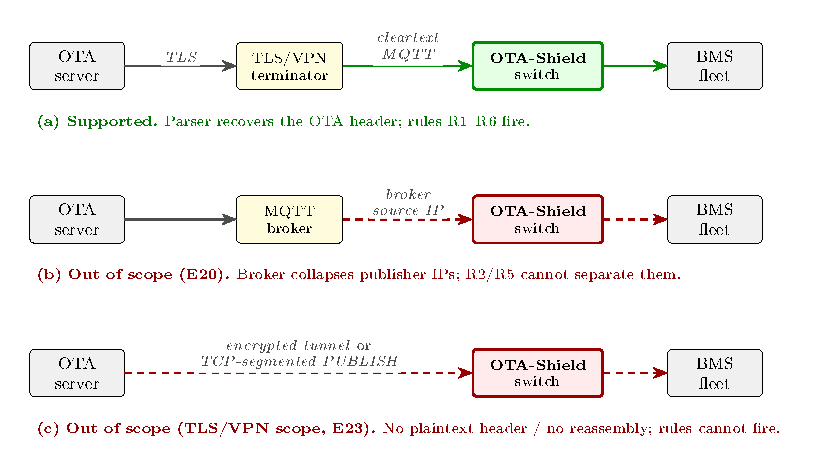
\includegraphics[width=0.82\textwidth]{figures/deployment_scope.pdf}
  \caption{Deployment scope, fixed by the threat model. \otashield{} is
  supported only on a cleartext MQTT segment after TLS or VPN termination
  (a), where the parser recovers the OTA header and rules R1--R6 fire. Two
  paths are outside the evaluated build: (b) a brokered path, where the
  broker rewrites every PUBLISH to its own source IP and the source-based
  rules can no longer separate publishers (evaluated as a negative control
  in E20, \S\ref{sec:e20-broker}); and (c) an encrypted tunnel that reaches
  the switch intact, or a PUBLISH split across TCP segments, where no single
  packet presents a parseable header and the data plane performs no
  reassembly (E23, \S\ref{sec:e23-tcp}). Dashed red paths mark unsupported
  placements, not demonstrated capability.}
  \label{fig:scope}
\end{figure*}

%% ====================================================================
\section{Related Work}\label{sec:related}

We organize prior work by what each line of research can express, the
assumptions it makes, and the limitation that leaves the OTA
fleet-coordination problem open.

\paragraph{In-network security on programmable switches.}
Programmable-switch security work can enforce per-packet policy at
line rate, but the published targets are volumetric or generic. Most
P4/Tofino work targets volumetric DDoS: Poseidon compiles declarative
defenses~\cite{zhang2020poseidon}, Jaqen reaches 380~Gb/s with
sketch-based mitigation~\cite{liu2021jaqen}, Patronum adds per-flow
state~\cite{wu2024patronum}, AlSabeh et al.\ run entropy-based
DPI~\cite{alsabeh2022p4ddpi}, and ACC-Turbo handles pulse-wave
traffic~\cite{alcoz2022accturbo}. Beyond DDoS, Kang et al.\ enforce
context-aware enterprise access-control policies (BYOD) in the data
plane without a control-plane round-trip~\cite{kang2020poise}, and
Xing et al.\ mitigate network covert channels at line rate while
preserving TCP performance~\cite{xing2020netwarden}; both confirm that
the programmability benefit reaches policy-enforcement and
behavioral-anomaly problems beyond volumetric attacks. A parallel line
pushes flow-level machine learning into the data
plane~\cite{samsonraj2025dddas,chen2024p4nids,mittal2024cybersentinel}.
The closest methodological neighbor is Bui et
al.~\cite{binh2026p4mqtt}, which parses MQTT in P4 on the BMv2
software target and enforces topic-prefix authorization with 99.8\%
accuracy and sub-ms latency. Its assumption set differs from ours on
platform, domain, threat model, policy model, stateful scope, and
evaluation rigor; Table~\ref{tab:bui-compare} marks the six axes. None
of this prior work targets OTA firmware attacks on grid
infrastructure.\label{sec:related-bui}

\begin{table}[pos=htbp]
  \centering
  \caption{Axis-by-axis comparison with Bui et
  al.~\cite{binh2026p4mqtt}.}
  \label{tab:bui-compare}
  \footnotesize
  \begin{tabular}{@{}p{0.20\columnwidth}p{0.32\columnwidth}p{0.36\columnwidth}@{}}
    \toprule
    \textbf{Axis} & \textbf{Bui et al.} & \textbf{\otashield{}} \\
    \midrule
    Target platform
      & BMv2 software reference; no MAU budget or PHV layout
        constraints.
      & \tofino{} hardware; reports measured layout against the
        12-stage MAU budget, 48-byte digest quantum, and register
        restrictions (\S\ref{sec:design}). \\
    \addlinespace
    Target domain
      & Generic edge-IoT MQTT anomalies.
      & BESS firmware distribution on a grid-operator path
        (\S\ref{sec:background}). \\
    \addlinespace
    Threat model
      & Endpoint compromise and topic-ACL abuse.
      & Channel compromise with valid signing material and authorized
        topics, fleet-coordinated campaigns. \\
    \addlinespace
    Policy model
      & Stateless topic-prefix authorization.
      & RAT with Gate~A and Gate~B arbitration
        (Alg.~\ref{alg:rat-gate}) over per-BMS rollout context. \\
    \addlinespace
    Stateful scope
      & Session-level flow state.
      & Per-BMS version high-water (R6) and Bloom-gated fleet-fanout
        counter (R5). \\
    \addlinespace
    Evaluation rigor
      & 99.8\% enforcement on software-timed BMv2.
      & Hardware latency (median
        $\approx$\EEightstochasticLatencyMedianMs{}\,ms,
        p95~$\approx$\EEightstochasticLatencyPninefiveMs{}\,ms),
        bootstrap F1 CIs over 20 stochastic trials, ablation
        (\S\ref{sec:e4}), adversarial-boundary sweep (\S\ref{sec:e9}),
        Suricata/Zeek baseline on identical traffic
        (\S\ref{sec:e10}). \\
    \bottomrule
  \end{tabular}
\end{table}

\paragraph{OTA firmware security and BESS prior work.}
This line of work secures the firmware after it arrives, which leaves
fleet-wide coordination during distribution invisible. Firmware-update
attacks on IoT devices are well
documented~\cite{verderame2023pariot,nikbakht2022rosym}; AoT shows
replay and rollback on real devices~\cite{oh2025fota5g};
SUIT~\cite{rfc9019} and Uptane~\cite{lorch2024uptane} standardize
cryptographic signing; and DDoSViT~\cite{ali2025ddosvit} defends the
OTA channel from disruption. All of these verify firmware after
delivery, so fleet-wide coordination during distribution is invisible
to them. On the BESS side, \"{O}hrstr\"{o}m et~al.\ give the first
cloud-BESS attack reference model~\cite{ohrstrom2025balance}, Trevizan
et~al.\ catalogue BESS risks and controls~\cite{trevizan2022bess},
Culler et~al.\ observe active scanning of exposed BMS
interfaces~\cite{culler2025threatlandscape}, and GAN/ensemble
detectors run on-device over telemetry~\cite{islam2023cascading}. The
NERC~RSTC white paper recommends in-network visibility as a
compensating control for small DERs outside mandatory CIP scope;
\otashield{} fills that gap on switching silicon.

\paragraph{Threshold derivation and CPU-based IDS baselines.}
A CPU-based signature IDS has the throughput but not the arbitration
needed for this problem. IDS anomaly thresholds are usually set from
measured baseline distributions rather than expert
heuristic~\cite{almalawi2020addon,sharafaldin2018cicids,cai2015cusumewma};
we follow the same P99$+k\sigma$ pattern on a 90-minute on-testbed
trace (\S\ref{sec:eval}). Suricata and Snort remain the reference
open-source ICS IDS~\cite{waleed2022whichids}, and Suricata reaches
tens of~Gb/s via AF\_PACKET~\cite{hu2019analysinghighspeed}, well
above the OTA-channel loads here. The meaningful question is therefore
not throughput but expressiveness: whether the rule language can
capture stateful, RAT-aware arbitration. \S\ref{sec:eval} answers that
directly on identical traffic.

%% ====================================================================
\section{System Design}\label{sec:design}

\otashield{} splits detection between a \tofino{} data plane that
enforces per-packet rules inside the ASIC pipeline and a Python
control plane that arbitrates ambiguous detections against a
Rollout-Authorization Table (RAT). This subsection describes what each
component does, why it is needed, and the constraint it addresses; the
hardware realization follows in \S\ref{sec:impl}.

\subsection{Architecture overview}

Fig.~\ref{fig:arch} shows the split. The data plane carries the
always-on, per-packet work: it parses the OTA header and evaluates the
detection rules at forwarding speed, where a coordinated campaign's
fanout shape is exposed. The control plane carries the slower,
policy-aware work: it holds the rollout schedule and decides whether a
flagged event belongs to an authorized rollout or to an attack. The
split is needed because the campaign-versus-attack decision requires
state (the rollout schedule) and matching logic that do not fit the
per-packet ASIC budget, while the cheap campaign-shape signal must run
on every packet without a control-plane round-trip.

\begin{figure*}[pos=htbp]
  \centering
  
\includegraphics[width=0.85\textwidth]{figures/system_architecture.pdf}
  \caption{System architecture. The data plane (left) processes every
  packet through five detection rules (R1, R2, R4, R5, R6), backed by
  per-BMS state registers including an R6 version high-water mark;
  digests stream to the control plane (right) via gRPC; the RAT
  arbiter installs session overrides (5-tuple-keyed by default; a
  source-IP aggregation variant is preserved as a compile-time knob,
  see~\S\ref{sec:e13}) with a 5\,s fail-closed TTL. Gate~A and Gate~B
  (\S\ref{sec:rat-gates-6a}--\ref{sec:rat-gates-6b}) run inside the
  arbiter.}
  \label{fig:arch}
\end{figure*}

\subsection{Detection rules}\label{sec:rules}

Each rule answers one attack pattern from
\S\ref{sec:background}. R2 (unauthorized source) is an identity check
on the firmware source IP against the operator's allow-list; its input
is the IPv4 source address and its output is a terminal fire when the
address is absent, implementing a fail-closed policy. R4 (oversize)
compares the cumulative session byte count against the maximum
legitimate firmware size; it is terminal because no authorized image
exceeds that bound. R5 (fleet fanout) counts the distinct destination
BMS addresses an \emph{unauthorized} source reaches inside a
60-second window; its counter is gated on the unauthorized-source flag
(\texttt{r2\_fired}), so on the deployed build it charges only behind the
terminal R2 drop and functions as a fanout telemetry signal rather than
an independent verdict (\S\ref{sec:cascade-fix}). R6 (version rollback) compares the OTA-header version
against a per-BMS high-water mark and fires when the observed version
is strictly lower, which catches a signed-but-older image that
endpoint signature verification accepts. R1 (rapid replay) measures
the inter-update interval per BMS and fires when it falls below a
cadence threshold; it is enabled only when per-BMS cadence is slower
than $\tau_{\mathrm{R1}}$.

With compile-time thresholds $\tau_{\mathrm{R1}}$, $\tau_{\mathrm{R4}}$,
$\tau_{\mathrm{R5}}$, the three threshold-bearing rules fire when
\begin{align*}
  \text{R1 fires if}\; & \Delta t_i < \tau_{\mathrm{R1}}, \\
  \text{R4 fires if}\; & B_i > \tau_{\mathrm{R4}}, \\
  \text{R5 fires if}\; & C_W > \tau_{\mathrm{R5}},
\end{align*}
where $\Delta t_i$ is the inter-update interval for BMS~$i$, $B_i$ is
the session byte count for session~$i$, and $C_W$ is the count of
distinct destination BMS addresses inside the R5 window $W$. R2 fires
when the source IP is not in the authorized-source allow-list, and the
OTA-header sanity checks are handled by the control plane. R6 fires
when the observed OTA-header version $v_i$ is strictly less than the
stored per-BMS high-water mark $v^{\star}_i$. R5's fleet-fanout count
is charged only against unauthorized sources, so an authorized fleet
rollout does not consume the detector's fanout budget; the
implementation gates the count update on the R2 fire flag
(\S\ref{sec:impl}).

\subsection{Policy engine and RAT-aware arbiter}\label{sec:policy}

The policy engine splits enforcement into a fast data-plane verdict
and a slower control-plane arbitration. In the data plane, the policy
control block (Fig.~\ref{fig:policy}) combines per-rule fire flags
into a byte-wide action code. R2 (unauthorized source) drops the
packet at the deparser. A behavioral rule fire (R1, R4, or R6) sets a
\texttt{HOLD} action code and emits a \texttt{hold\_digest} to the
controller. The controller then decides: R4 stays terminal, while R1
and R6 go through the two-stage RAT arbiter
(\S\ref{sec:rat-gates-6a}--\ref{sec:rat-gates-6b}), which either
installs a \texttt{session\_allow} override (via Gate~A or Gate~B) or a
\texttt{session\_deny}. R5 is r2-gated: it co-fires with R2 (terminal
DROP) and otherwise contributes a fleet-fanout flag to the digest rather
than a distinct arbiter path. Packets that fire no rule pass with action
code zero and no digest.

\begin{figure*}[pos=htbp]
  \centering
  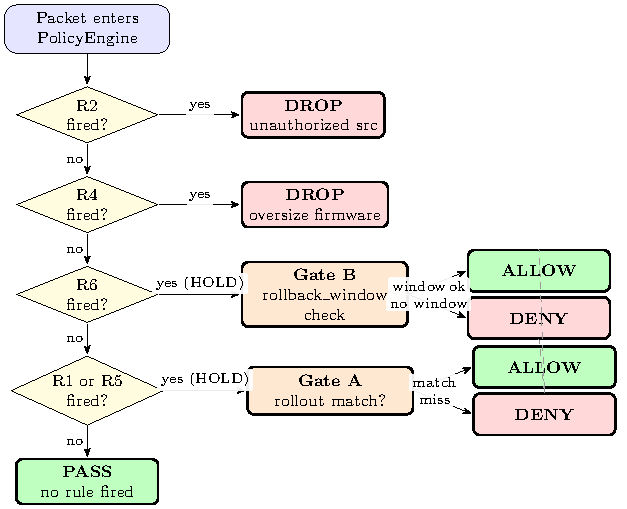
\includegraphics[width=0.72\textwidth]{figures/policy_flowchart.pdf}
  \caption{Policy decision flowchart. All rule fires emit a
           \texttt{hold\_digest} to the controller. R2 (unauthorized
           source) and R4 (oversize payload) remain terminal DROP
           decisions. R1 (rapid replay) and R6
           (version rollback) enter control-plane arbitration: Gate~A
           demotes an R1 fire that matches an active authorized
           rollout to PASS (R5 cannot reach Gate~A on the deployed build,
           its counter being r2-gated, \S\ref{sec:cascade-fix}), and
           Gate~B demotes an R6 fire to PASS only
           when the active RAT entry carries an explicit
           \texttt{rollback\_window} covering the observed version. Any
           other HOLD becomes a DROP override. Override entries expire
           after 5\,s (fail-closed).}
  \label{fig:policy}
\end{figure*}

Packets with \texttt{action\_code} $\neq$ 0 generate a
\texttt{hold\_digest} (28~bytes, well under \tofino{}'s 48-byte learn
quantum) carrying the 5-tuple, session ID, BMS index, all five
rule-fire flags, and the OTA version and size. The controller compares
this digest against the RAT manifest (Table~\ref{tab:rat}); a match
installs a \texttt{session\_allow} override, a miss installs
\texttt{session\_deny}. Both expire via a 5-second timer, giving
fail-closed recovery if the controller stalls. Because the digest carries
the BMS index and all five rule-fire flags, every detection is localized
to a specific device and rule rather than reported only in aggregate, in
the manner of localization-aware ICS detectors~\cite{lin2018tabor}; the
per-strategy, per-rule breakdown this enables is reported for the mimicry
sweep in \S\ref{sec:e21}.

\begin{table*}[pos=htbp]
  \centering
  \caption{Rollout-Authorization Table fields. The manifest is a
  per-rollout JSON object loaded by the controller; a HOLD packet
  passes only when every condition matches.}
  \label{tab:rat}
  \footnotesize
  \begin{tabular}{@{}l p{0.70\textwidth}@{}}
    \toprule
    Field & Policy semantics \\
    \midrule
    \texttt{authorized\_source\_ips}  & Allow-list of IPv4 addresses
        permitted to originate firmware PUBLISHes for this rollout. \\
    \texttt{target\_bms\_list}        & Allow-list of destination BMS
        IPs within scope of the rollout. \\
    \texttt{valid\_window\_start/end} & UTC wall-clock window during
        which the rollout is active. \\
    \texttt{expected\_payload\_size\_range} & Inclusive byte range for
        advertised firmware size. \\
    \texttt{expected\_firmware\_version}    & Version number reported in
        the OTA header for control-plane sanity check. \\
    \texttt{max\_concurrent\_targets} & Enforced per-rollout cap on the
        number of concurrent active sessions a rollout may hold; the
        controller denies admission beyond it (0~$=$~unlimited). \\
    \texttt{rollback\_window}         & Optional
        \{\texttt{min\_version}, \texttt{max\_version}\} pair
        authorizing a rollback range for this rollout
        (see \S\ref{sec:rat-gates-6b}). Default-absent: R6 remains a
        terminal rule. \\
    \bottomrule
  \end{tabular}
\end{table*}

\subsubsection{Gate~A: RAT-gated demotion of R1 fires}\label{sec:rat-gates-6a}

Gate~A relaxes R1 (rapid replay) for packets that belong to an
authorized rollout. Two stages run per HOLD digest. Stage one keeps R2
(unauthorized source) and R4 (oversize payload) terminal: any
combination flagged as terminal installs \texttt{session\_deny}. Stage
two looks at R1 fires against the active RAT entries. R5 (fleet fanout)
does not reach this gate on the deployed build: the data-plane R5
counter is gated on \texttt{r2\_fired}, so R5 only fires alongside R2 (an
unauthorized source), and stage one has already made that combination
terminal.

Notation: $r_1$, $r_2$, $r_4$, $r_5$, $r_6$ are the rule-fire flags;
$s$ the source IP; $d$ the destination BMS; $v$ the OTA-header version.
Gate~A demotes an R1-only fire to PASS when
$r_2\!=\!r_4\!=\!0$ and a RAT entry $R$ exists such that
$s \in R.\mathit{authorized\_source\_ips}$,
$d \in R.\mathit{target\_bms\_list}$, the current time lies inside
$R.\mathit{valid\_window}$, the advertised size lies inside
$R.\mathit{expected\_payload\_size\_range}$, and $v$ matches
$R.\mathit{expected\_firmware\_version}$ (or an immediate neighbour, to
tolerate staged major/minor bumps inside one rollout). The controller
then installs a \texttt{session\_allow} override instead of
\texttt{session\_deny}. On the benign workloads of \S\ref{sec:e12}
and~\S\ref{sec:e7}, Gate~A clears inter-update (R1) HOLDs on
authorized staged, emergency, and migration rollouts to zero-drop
outcomes, with no data-plane threshold retuned.

\subsubsection{Gate~B: RAT-gated demotion of R6 fires}\label{sec:rat-gates-6b}

Gate~B relaxes R6 (version rollback) only when the RAT explicitly
authorizes the downgrade. R6 follows the same shape as Gate~A but
through a parallel rollback gate. An R6-only fire ($r_6\!=\!1$,
$r_2\!=\!r_4\!=\!0$, no other terminal rule co-fired) is demoted to
PASS only when a matching RAT entry $R$ exists (same
source/destination/window/size checks as Gate~A), $R$ carries an
explicit \texttt{rollback\_window} field, and $v$ lies inside the
range $[R.\mathit{min\_version},\,R.\mathit{max\_version}]$ that the
window advertises. If any check fails, R6 stays terminal and the
controller installs \texttt{session\_deny}.

The default is closed. A RAT entry that omits
\texttt{rollback\_window} leaves R6 as a terminal HOLD/DROP rule, so a
deployment that never authorizes a downgrade sees the same attack
surface it had before. The gate exists to cover operator-authorized
emergency rollbacks (for instance, an OEM recall that moves a fleet
from version~48 back to version~47), while the data-plane monotonicity
check still fires on every unauthorized downgrade.

\begin{algorithm}[!ht]
\footnotesize
\caption{Two-stage RAT-aware arbiter (Gate~A and Gate~B).}
\label{alg:rat-gate}
\begin{algorithmic}[1]
\Require digest $D$ with flags $r_1,r_2,r_4,r_5,r_6$, source $s$,
         destination $d$, size $b$, version $v$; RAT manifest $\mathcal{R}$.
\If{$r_2 = 1$ \textbf{or} $r_4 = 1$} \Comment{terminal}
  \State \Return \texttt{session\_deny}
\EndIf
\State $R \gets \mathrm{MatchRAT}(\mathcal{R}, s, d, b, \mathit{now})$
\If{$R = \varnothing$}
  \State \Return \texttt{session\_deny}
\EndIf
\If{$r_6 = 1$} \Comment{Gate~B: default-closed}
  \If{$R.\mathit{rollback\_window}$ exists \textbf{and}
      $v \in R.\mathit{rollback\_window}$}
    \State \Return \texttt{session\_allow}
  \Else
    \State \Return \texttt{session\_deny}
  \EndIf
\EndIf
\If{$r_1 = 1$} \Comment{Gate~A ($r_5$ unreachable: gated on $r_2$)}
  \State \Return \texttt{session\_allow}
\EndIf
\State \Return \texttt{session\_deny} \Comment{unreachable under digest precondition}
\end{algorithmic}
\end{algorithm}

\noindent Gate~A handles rollout-context demotion for R1;
Gate~B handles explicit rollback authorization for R6.
$\mathrm{MatchRAT}$ checks source, destination, time window, and size
range; it does not require exact version equality, which would reject
legitimate staged major/minor bumps inside an active campaign.
The final \texttt{session\_deny} is unreachable on well-formed input:
the data plane emits \texttt{hold\_digest} only when $r_1 \lor r_2 \lor
r_4 \lor r_5 \lor r_6 = 1$. The guards at lines~2--4 and~9 remove
$r_2$, $r_4$, and $r_6$, and Gate~A removes $r_1$. The one remaining
case, an $r_5$-only fire, cannot occur on the gated build: the R5
counter is gated on \texttt{r2\_fired}, so every $r_5$ fire also sets
$r_2$ and is already caught by the terminal guard. It is retained as a
defensive default for malformed or replayed digests. Every arbiter decision is logged, and all reported
classification verdicts are read directly from this decision log.

%% ====================================================================
\section{Implementation}\label{sec:impl}

This section describes the \tofino{} realization of the design: the
ingress pipeline that evaluates the rules, and the controller that runs
the arbiter.

\subsection{P4 ingress pipeline}

The ingress pipeline (Fig.~\ref{fig:pipeline}) comprises a
protocol-aware parser and nine MAU-stage control blocks, within the
12-stage \tofino{} budget.

\begin{figure*}[pos=htbp]
  \centering
  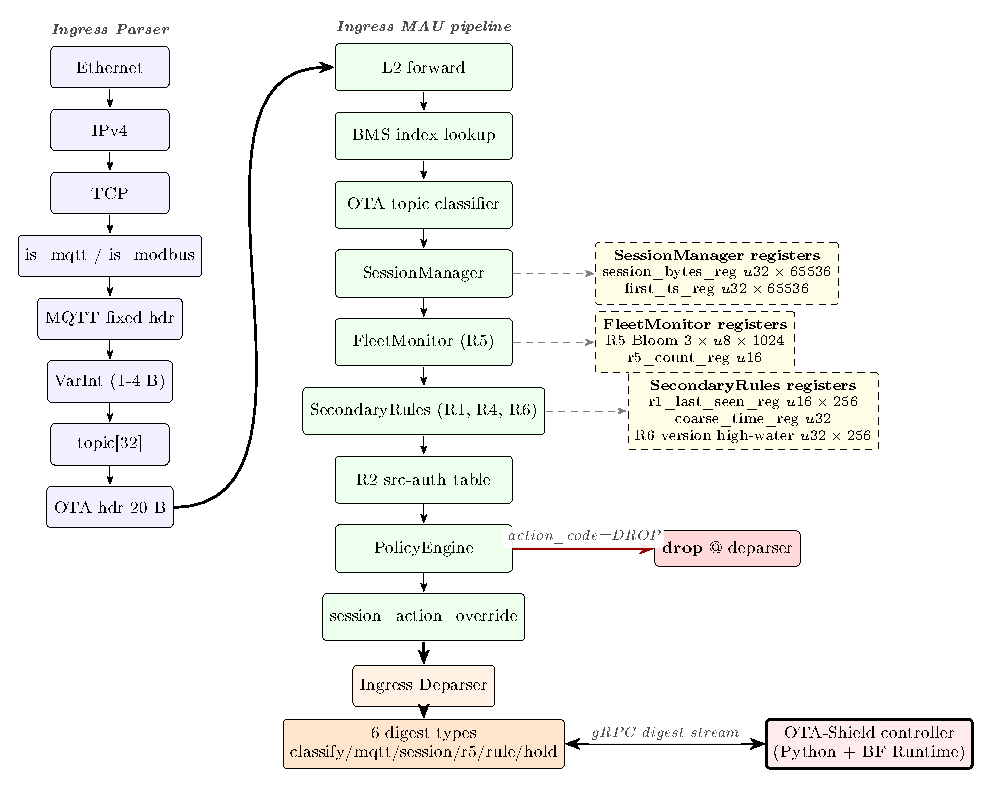
\includegraphics[width=0.95\textwidth]{figures/p4_pipeline.pdf}
  \caption{P4 ingress pipeline. Dashed arrows connect MAU control
  blocks to their stateful registers. Topic and OTA header use
  fixed-size slots; other parameter combinations are discussed in
  \S\ref{sec:e18}.}
  \label{fig:pipeline}
\end{figure*}

\paragraph{Parser.} The ingress parser identifies MQTT traffic on TCP
port~1883. For MQTT PUBLISH packets (\texttt{mtype}=3), it extracts the
variable-length remaining-length field (1--4 bytes), a 32-byte
null-padded topic slot, a QoS-1 packet identifier, and the first
20~bytes of the payload as the OTA header. The OTA header carries a
4-byte magic (\texttt{0x4F544153} = ``OTAS''), a 4-byte firmware
version, a 4-byte advertised size, and an 8-byte hash hint. All
metadata fields are byte-aligned (\texttt{bit<8>}) to satisfy
\tofino{}'s PHV allocator constraints.

\paragraph{Session manager.} A CRC32 hash of the 5-tuple produces a
16-bit session index into two 65\,536-entry registers:
\texttt{session\_bytes\_reg} (cumulative TCP payload bytes) and
\texttt{session\_first\_ts\_reg} (first-seen timestamp with a non-zero
sentinel). On TCP FIN or RST, a read-and-clear action atomically
returns the session summary and resets the slot.

\paragraph{Fleet monitor (R5).} Three independent Bloom filters (1024
entries each, CRC32 / CRC16 / CCITT hashes with salt bytes) track
distinct destination BMS addresses within a 60-second tumbling window.
A single \texttt{RegisterAction} on a 16-bit counter increments on
Bloom miss and returns the current count. A range-match table fires R5
when the count exceeds the threshold (compile-time constant,
default~4). The controller clears all three Bloom registers and the
counter every 60 seconds. Bloom inserts and the count update are gated
on \texttt{r2\_fired==1} so authorized fleet rollouts do not consume
Bloom slots; only unauthorized fanout charges against the detector.
This Bloom-sizing assumption is revisited in~\S\ref{sec:bloom-scaling}
for fleet-scale deployments.

\paragraph{Secondary rules (R1, R4).} R1 uses a 256-slot 16-bit
register indexed by BMS number. The stateful ALU computes
\texttt{coarse\_time\_sec\_lo -- last\_seen} as the inter-update delta;
a range-match table fires R1 when the delta is below the threshold
(compile-time constant, derived from the E7 baseline as 14\,400~s =
4~h; see \S\ref{sec:e7}). R4 compares the upper 16 bits of
\texttt{session\_bytes\_val} against a range threshold (compile-time
constant, derived from E7 as 32 units of 64~KiB = 2~MiB). R2 is an
exact-match table on \texttt{ipv4.src\_addr}: entries for authorized
OTA sources are installed by the controller at startup from the RAT
manifest. The default action fires R2, implementing a fail-closed
policy.

\paragraph{Version rollback (R6).} R6 keeps a per-BMS firmware-version
high-water mark in a 256-slot 32-bit register indexed by BMS number.
The stateful ALU compares the incoming OTA-header version against the
stored mark, fires R6 when the observed version is strictly below it,
and raises the slot to the maximum of the two values. There is no
threshold to tune: the check is version-monotonic and catches
signed-but-older firmware that endpoint signature verification lets
through. An R6 fire emits a \texttt{hold\_digest}, and the control
plane decides. Gate~B consults the RAT and clears the fire only when an
authorized rollback entry is active.

\paragraph{Compile-time thresholds.} All thresholds are compile-time
constants (range-match table entries) rather than runtime registers,
for two reasons. First, a runtime register comparison would need two
runtime operands in the same MAU action, which the \tofino{} gateway's
predicate-width constraint disallows. Second, the thresholds are
derived once per deployment from an E7-equivalent baseline
(\S\ref{sec:e7}) and are not intended to drift; pinning them at compile
time makes their provenance auditable and excludes a silent-override
vector on the control plane. Re-deriving thresholds for a new
deployment profile is a P4 recompile (minutes), not a runtime
reconfiguration.

\subsection{Controller}

The controller attaches to the switch over local-loopback gRPC. It
installs R2 allow-list entries and Bloom-clear timers at startup,
receives each \texttt{hold\_digest}, and runs the two-stage arbiter of
\S\ref{sec:policy} on every HOLD. A match installs a
\texttt{session\_allow} override on the 5-tuple-keyed
\texttt{session\_action\_override} table; a miss installs
\texttt{session\_deny}. Both expire after a 5-second fail-closed TTL.
The controller loads the RAT manifest at startup and on hot-reload,
verifies its ed25519 signature when run under
\texttt{--require-signed-rat}, and retains the last-known-good manifest
when a reload fails verification.

%% ====================================================================
\section{Evaluation}\label{sec:eval}

This section answers five research questions about \otashield{} with
the testbed and methodology described in
\S\ref{sec:testbed}--\ref{sec:methodology}.

\noindent\emph{Main result map.} The evaluation has five load-bearing
results. E8 reports the headline designed-family detection result; E12 tests
whether authorized rollouts are admitted without false drops; E19 and
\Enineteenp{} isolate the rollback rule and its first-contact limitation; E21
measures adaptive mimicry as the main adversarial blind zone; and E10 compares
\otashield{} against CPU-based IDS baselines on identical traffic. The remaining
experiments are support, boundary, or artifact-provenance checks, and the
\emph{Role} column of Table~\ref{tab:results} marks each one.

\begin{itemize}
  \item \textbf{RQ1.} Does the detector classify attack and benign OTA
    events correctly on the reference testbed? (E1, E2, E6, E8, E12,
    E12b.)
  \item \textbf{RQ2.} Is the RAT-aware arbiter necessary, and is R6 the
    sole detector of unauthorized rollback? (E4, E19, \Enineteenp{}.)
  \item \textbf{RQ3.} How does each rule degrade under adversarial
    mimicry, threshold sweeps, and long-horizon slow-cadence traffic?
    (E9, E21, E7b.)
  \item \textbf{RQ4.} How does \otashield{} compare to CPU-based IDS
    baselines on identical traffic? (E10 variants i--vii.)
  \item \textbf{RQ5.} What latency, throughput, capacity, and
    portability costs does the deployment pay? (E14, E11, E13, E18.)
\end{itemize}

Every result below is measured on one deployed configuration, summarized in
Table~\ref{tab:final-build}; Table~\ref{tab:coverage} maps each attack
pattern to the rule that answers it and to that rule's measured blind zone.

\begin{table}[pos=htbp]
  \centering
  \caption{Final evaluated build. All results in this section are measured
  on this single deployed configuration.}
  \label{tab:final-build}
  \footnotesize
  \begin{tabular}{@{}ll@{}}
    \toprule
    Component & Final setting \\
    \midrule
    R5 gating            & r2-gated (counts unauthorized-source fanout only) \\
    Override table       & 5-tuple-keyed default; source-IP aggregation optional \\
    Per-source hold gate & inert (arms on R5 only, which is r2-shadowed) \\
    OTA profile          & cleartext MQTT reference profile (TCP/1883) \\
    Parser               & 32-byte null-padded topic slot + 20-byte OTA header \\
    Fleet                & 50 BMS emulated endpoints \\
    \bottomrule
  \end{tabular}
\end{table}

\begin{table*}[pos=htbp]
  \centering
  \caption{Rule/attack coverage on the final evaluated build. Each rule
  answers one attack pattern; the rightmost column states the measured
  blind zone.}
  \label{tab:coverage}
  \footnotesize
  \begin{tabular}{@{}lllll@{}}
    \toprule
    Attack pattern & Rule & Detected in final build? & Main evidence & Known blind zone \\
    \midrule
    Unauthorized firmware source & R2 & Yes, terminal DROP                    & E1, E8                  & brokered-MQTT source-IP collapse (E20) \\
    Oversize firmware image      & R4 & Yes, $\geq$2.0625~MiB                 & E6, E9                  & 2.0--2.0625~MiB quantization dead zone \\
    Coordinated fleet fanout     & R5 & Telemetry behind R2, not independent  & E9, \S\ref{sec:cascade-fix} & authorized-source fanout (out of scope) \\
    Signed version rollback      & R6 & Yes                                   & E19, \Enineteenp{}, E7b & first-contact cold-start \\
    Rapid replay                 & R1 & Cadence-dependent, non-central        & E1, E9                  & inter-update interval $>\tau_{R1}$ \\
    \bottomrule
  \end{tabular}
\end{table*}

Table~\ref{tab:results} indexes every experiment to the RQ it supports
and to the subsection in which it is reported.

\subsection{Testbed}\label{sec:testbed}

\begin{figure*}[pos=htbp]
  \centering
  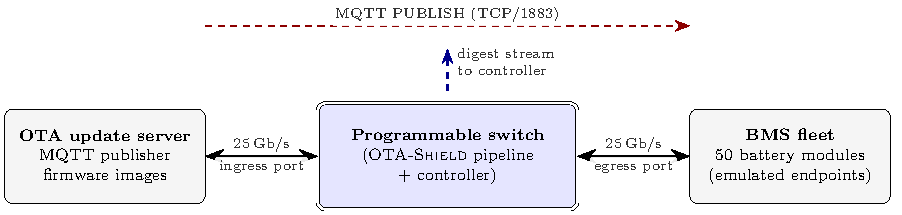
\includegraphics[width=0.8\textwidth]{figures/testbed_topology.pdf}
  \caption{Testbed topology. An OTA update server and a 50-unit BMS
  fleet connect to a programmable switch through data-plane links
  configured at 25\,Gb/s with RS-FEC (link capability; the experiments
  in this paper do not offer traffic at that rate). A separate
  management LAN carries control-plane gRPC traffic.}
  \label{fig:testbed}
\end{figure*}

The testbed (Fig.~\ref{fig:testbed}) consists of two commodity servers
bridged by a programmable switch. One server is the OTA update server,
publishing MQTT firmware messages. The other emulates a 50-unit BMS
fleet using network-layer aliases, so every unit appears on the wire as
a distinct endpoint. Both servers carry 25\,Gb/s network interfaces and
connect to the switch through RS-FEC links. The switch runs
BF-SDE~9.13.2, with the \otashield{} P4 pipeline loaded and the Python
controller attached over local-loopback gRPC.

Traffic generation is scripted: each scenario emits MQTT PUBLISH
packets carrying the 20-byte OTA header, records a wall-clock send
timestamp and a ground-truth label (\textsc{legit} or \textsc{attack}),
and writes the record to a per-trial log. The controller writes every
policy decision to a second log. We join the two logs by 4-tuple
(\texttt{src\_ip}, \texttt{dst\_ip}, \texttt{src\_port},
\texttt{dst\_port}) so each labelled event inherits the detector's
verdict.

\subsection{Methodology}\label{sec:methodology}

\paragraph{Trial independence.} Between trials the sweep driver signals
the controller, which re-seeds all R1 last-seen register slots, clears
the R5 Bloom filters and counter, and waits 70~s for the R5 window to
expire. Each trial starts from identical detector state.

\paragraph{Ground-truth labeling.} Labels are assigned by the scenario
generator, not by the detector. Events with no matching controller
decision or digest are counted as \textsc{no\_decision} rather than
silently dropped, preventing digest-transport loss from inflating
reported metrics.

\paragraph{Threshold derivation versus evaluation (E7).}\label{sec:e7}
Baseline traffic from the long-run benign trace is used only to derive
R5, R1, and R4 thresholds; it is never used to score detection metrics.
All reported precision, recall, F\textsubscript{1}, and latency numbers
come from separately generated evaluation scenarios (E1, E4, E6, E8,
E9, E10, E11) that the thresholds have not been exposed to. A
\EsevenNEvents{}-event Poisson baseline trace (${\approx}90$~min, mean
IAT~2~s) of authorized PUBLISHes reaches
random BMSes with firmware sizes drawn uniformly from 256~KiB--2~MiB.
From this baseline we compute three distributions: (a)~distinct-BMS
count per 60-second window (R5 metric), (b)~per-BMS inter-rollout
interval (R1 metric), and (c)~firmware size (R4 metric). The P99.9 tail
of the distinct-BMS count is \EsevenDistinctBMSPninenineNine{}
(legitimate fleet rollouts reach at most
$\approx$\EsevenDistinctBMSPninenineNine{} distinct BMS targets per
60-second window at P99.9), the P0.1 tail of the inter-rollout interval
is \EsevenIntervalPzeroOne{}~s (R1 minimum interval
\EsevenRoneRecommended{}~s), and the P99.9 firmware size is
\EsevenSizePninenineNine{}~B (R4 bound \EsevenRfourRecommended{}~B). R4
is pinned directly at the E7-derived $\approx$2\,MiB bound. R5 is a
compile-time constant set to 4 (fires when distinct-BMS count exceeds~4
per 60-s window), substantially below E7's P99.9 of
\EsevenDistinctBMSPninenineNine{}; R5 is intentionally tighter than the
baseline tail to target attacks reaching $\geq$5 distinct BMS targets,
a deliberate design choice for the 50-unit testbed scale, not a
threshold derived from the P99.9 tail. R1 is pinned looser
(14{,}400\,s vs.\ E7's P0.1) to reflect the update cadence of scheduled
campaigns rather than the minimum legal inter-message gap.

\paragraph{Deterministic versus stochastic experiments.}\label{sec:methodology-bounds}
Experiments with fixed seeds (E1, E4, E5, E6) function as correctness
tests; repeating a deterministic computation is not statistical
sampling, so they are reported without CIs. E8 introduces random seed,
BMS ordering, and inter-arrival jitter per trial; bootstrap 95\% CIs on
E8 are the paper's headline statistical result. \Enineteenp{}
(\EOneNineprollbackstochasticNTrials{}~trials,
\EOneNineprollbackstochasticEventTotal{}~events:
\EOneNineprollbackstochasticEventAttack{} rollback attacks and
\EOneNineprollbackstochasticEventLegit{} legitimate events) randomizes
per-BMS version ordering and inter-arrival jitter under a fixed top-level
seed. On the deployed gated build it yields zero benign false positives
(precision \EOneNineprollbackstochasticPrecisionMean{}, Wilson 95\% CI
[\EOneNineprollbackstochasticPrecisionCIlo{},
\EOneNineprollbackstochasticPrecisionCIhi{}]); the genuine between-trial
variance now lives in \emph{recall}, because a stochastic share of the
rollbacks are first-contact events that R6 structurally cannot catch on
the version it has never seen (\S\ref{sec:cascade-fix}). We therefore
report a strict recall that counts those first-contact misses
(\EOneNineprollbackstochasticRecallMean{}, Wilson 95\% CI
[\EOneNineprollbackstochasticRecallCIlo{},
\EOneNineprollbackstochasticRecallCIhi{}]) alongside the lenient figure
that excludes them
(\EOneNineprollbackstochasticRecallLenientMean{}). Because \otashield{}'s
rules apply hard compile-time thresholds with no tunable per-event score,
a swept precision--recall curve is degenerate (precision stays at 1.000
across the operating range), so we report precision, recall, and
F\textsubscript{$\beta$} at the deployed fixed-threshold operating point
and present the cross-detector trade-off as operating points on the
precision--recall plane (Fig.~\ref{fig:suricata}), the appropriate
presentation under the class skew here~\cite{davis2006prroc}. Where an
experiment observes
zero false positives or negatives we report a Clopper--Pearson
rule-of-three one-sided 95\% upper bound on the error rate
($\leq\RuleOfThreeSixHundred{}\%$ for E8,
$\leq\RuleOfThreeFourFifty{}\%$ for E12, i.e.\ at most 0.50\% and
0.67\% of events could be mislabelled at the 95\% confidence level
given the observed 0/N count); because these are correctness runs
rather than independent significance tests, a strict Bonferroni
correction is inappropriate. For E8 precision specifically, FP~$=$~0
across all 20 trials and 600 benign events; the bootstrap CI compresses
to a degenerate [1.000,\,1.000] and is replaced by the Clopper--Pearson
one-sided 95\% upper bound on FP rate of $\leq$\RuleOfThreeSixHundred{}\%
(= 3/600, identical to the rule-of-three bound).

\paragraph{Train/test discipline and capture duration.}\label{sec:leakage-discipline}
\otashield{} has no learned parameters. The rules are fixed thresholds and
the RAT is operator-supplied, so there is no train/test split to leak
across. We instead guard against the inflated-score failure mode that
afflicts learned ICS detectors~\cite{kus2022falsesense} in two ways.
First, the benign test set contains operationally \emph{unusual but
legitimate} events: emergency hotfix re-pushes, mid-rollout source
migration, delayed-retry bursts, and an authorized fleet rollback (E12).
A PASS verdict is therefore earned against traffic that superficially
resembles an attack, not against quiescent background. Second, the adversarial sweeps
(E9, E21, E23, E20) probe attack variants the rules were not hand-tuned
against, including sub-threshold mimicry and TCP segmentation, so the
reported coverage is on unseen behavior. The zero-false-positive bounds
above are tied to event counts rather than wall-clock duration; for
reference the benign captures span roughly 3.5~min (E8, 600 events) and
25~min (E12, 450 events) plus the longer signed-manifest soak of E12b. A
multi-hour production soak in the manner of Caselli et
al.~\cite{caselli2015specification} is future work; at the emulated
testbed's compressed cadence we report the event-count bound as primary.

\paragraph{Bootstrap for stochastic CIs.}\label{sec:cluster-bootstrap}
Stochastic experiments report 95\% confidence intervals from a
trial-level percentile bootstrap: per-trial point estimates
(precision, recall, F\textsubscript{1}) are resampled with replacement
over the $n$ trials, using $B = 2\,000$ replicates, and the 2.5th and
97.5th percentile of the resample distribution are reported as the CI
bounds. The confidence level is $\alpha = 0.05$. When all trials yield
the same point estimate the resulting distribution is degenerate; we
report the point in that case and instead quote the Clopper--Pearson
one-sided bound described above.

\begin{table*}[pos=htbp]
  \centering
  \caption{Experiment roadmap indexed by RQ. The \emph{Role} column tiers
  each experiment as \textsc{Primary} (a load-bearing claim: detection,
  admission, rollback, mimicry blind zone, or baseline), \textsc{Boundary}
  (a scope or blind-zone limit), \textsc{Support} (rule correctness,
  capacity, latency, or cost), or \textsc{Artifact} (manifest-lifecycle and
  build-provenance evidence). Rows marked $\dagger$ use
  the trial-level percentile bootstrap of \S\ref{sec:cluster-bootstrap};
  rows marked $\ddagger$ use Wilson 95\% CIs (or the Clopper--Pearson
  rule-of-three one-sided bound on zero-event cells); remaining rows are
  deterministic point counts. Deterministic trials (E1, E4, E6, E10)
  yield identical outcomes by construction; E11, E12, E13, E21, E18
  report per-event or per-scenario counts rather than classification
  F\textsubscript{1}.}
  \label{tab:results}
  \footnotesize
  \begin{tabular}{@{}l l l c l l l@{}}
    \toprule
    Exp.\ & Purpose & Type & Trials & RQ & Role & Headline \\
    \midrule
    E1  & Correctness (attack detection)   & deterministic & \EOneattackdetectionNTrials & RQ1 & Support  & F\textsubscript{1}~=~\EOneattackdetectionFOneMean \\
    E2$^{\ddagger}$  & FP baseline         & deterministic & 5                           & RQ1 & Support  & 0 FP \\
    E4  & RAT arbiter ablation             & deterministic & \EFourablationNTrials       & RQ2 & Support  & F\textsubscript{1}~=~\EFourablationFOneMean \\
    E6  & Oversized firmware (R4)          & deterministic & \ESixaFouroversizeNTrials   & RQ1 & Support  & F\textsubscript{1}~=~\ESixaFouroversizeFOneMean \\
    E8$^{\dagger}$  & Stochastic IID trials & stochastic   & \EEightstochasticNTrials    & RQ1 & Primary  &
        F\textsubscript{1}~=~\EEightstochasticFOneMean{} [\EEightstochasticFOneCIlo{}, \EEightstochasticFOneCIhi{}] \\
    E9  & Adversarial evasion sweeps       & deterministic & 3 $\times$ 4                & RQ3 & Boundary & boundary maps \\
    E10 & Suricata/Zeek baseline           & deterministic & 1 (PCAP replay)             & RQ4 & Primary  & see \S\ref{sec:e10} \\
    E11 & Controller digest-channel rate   & stress run    & 1                           & RQ5 & Support  & \ElevenAggregateLossPct{}\% aggregate loss \\
    E12$^{\ddagger}$ & Benign rollout stress & stress run  & 3                           & RQ1 & Primary  & 0 DROP on \EOneTwobenignrolloutScenarioTotal{} legit events \\
    E13 & Override-table capacity          & stress run    & 1                           & RQ5 & Support  & sat.\ at 4--8~s \\
    E14$^{\dagger}$ & Latency stage breakdown & post-hoc   & on E8                       & RQ5 & Support  & stage~1 p95 41.8~ms \\
    E21 & Per-strategy mimicry             & deterministic & \EOneSevenmimicryNTrials{}  & RQ3 & Primary  & \EOneSevenmimicryStrategyCatchPct\% coverage (\S\ref{sec:e21}) \\
    E18 & Reference-channel portability    & deterministic & 1                           & RQ5 & Boundary & \EeighteenMfourParsed/\EeighteenMfourVariants{} variants parse \\
    E19 & R6 rollback ablation             & deterministic & \EOneNinerollbackNTrials    & RQ2 & Primary  & F\textsubscript{1}~=~\EOneNinerollbackFOneMean{} with R6; collapses without R6 (\S\ref{sec:e19}) \\
    E12b$^{\ddagger}$ & Signed-manifest fail-safe & stress run & \EOneTwobsignedNTrials   & RQ1 & Artifact & last-known-good (LKG) pass-rate~=~100\% under sig-tamper (\S\ref{sec:e12b}) \\
    E7b$^{\ddagger}$ & Long-horizon slow cadence & \EsevenbDurationHours{}~h trace & 1    & RQ3 & Support  & R6 recall \EsevenbTPR{}, precision \EsevenbOverallPrecision{} (\S\ref{sec:e7b}) \\
    E23 & TCP-segmentation evasion         & deterministic & 250                         & RQ3 & Boundary & header-split evades all rules (\S\ref{sec:e23-tcp}) \\
    E20 & Brokered-MQTT topology           & deterministic & 80                          & RQ3 & Boundary & IP-collapse drops benign fleet (\S\ref{sec:e20-broker}) \\
    \bottomrule
  \end{tabular}
\end{table*}

\subsection{RQ1: Correctness on the reference testbed}\label{sec:rq-detection}

\noindent\textit{Finding: rules fire only where they should, and the
arbiter never drops an authorized rollout, including under stochastic
perturbation and signed-manifest tampering.}

The first block of experiments checks four things: that each rule fires
exactly on its designed trigger, that the arbiter returns the intended
verdict on every event, that stochastic perturbation does not collapse
those guarantees, and that the benign dual (the arbiter must not drop
authorized rollouts) holds end-to-end.

\paragraph{E1: attack detection.} Each trial sends 30 baseline
legitimate PUBLISHes, 30 rapid replays to the same BMSes (R1 fires; the
replay source is authorized, so R2 does not fire and R5's r2-gated counter
never runs), and 30 unauthorized-source PUBLISHes (R2 fires), 90~events.
Across \EOneattackdetectionNTrials{} trials, every trial produces
precision~\EOneattackdetectionPrecisionMean{},
recall~\EOneattackdetectionRecallMean{},
F\textsubscript{1}~=~\EOneattackdetectionFOneMean{}. Each rule fires
correctly on its designed trigger and the RAT arbiter classifies every
event as intended.

\paragraph{E2: false-positive baseline.} 50 authorized PUBLISHes per
trial (all \textsc{legit}), 5~trials. No false positives.

\paragraph{E6: R4 oversize detection.} A single MQTT session pushes
2.125~MiB of TCP payload (above the 2~MiB threshold). R4 fires
deterministically on all 3~trials.

\paragraph{Stochastic detection performance (E8).}\label{sec:e8}
E8 mirrors the E1 scenario but introduces realistic stochasticity:
random BMS ordering, Poisson inter-arrival times (mean 100~ms), and
ephemeral source ports drawn uniformly from 49152--65535. Each of
\EEightstochasticNTrials{} trials uses a distinct random seed,
producing independent draws. Across the \EEightstochasticNTrials{}
trials we observe precision~=~\EEightstochasticPrecisionMean{}
(FP~$=$~0/600 benign events; CP 95\% UB on FP rate
$\leq$\RuleOfThreeSixHundred{}\%; bootstrap CI degenerate),
recall~=~\EEightstochasticRecallMean{}
[\EEightstochasticRecallCIlo{}, \EEightstochasticRecallCIhi{}],
F\textsubscript{1}~=~\EEightstochasticFOneMean{}
[\EEightstochasticFOneCIlo{}, \EEightstochasticFOneCIhi{}] (trial-level
percentile bootstrap 95\% CIs, $B = 2\,000$ resamples). The 20-trial
sample size was chosen so that the bootstrap CI half-width for
F\textsubscript{1} is below 0.01, verified by plotting CI width as a
function of trial count from~5 to~20; the width plateaus by trial~15.
Per-trial F\textsubscript{1} dispersion is tight (interquartile range
within the CI, Fig.~\ref{fig:per_exp}), consistent with the low
missed-event rate on this workload; the pooled confusion matrix is
Fig.~\ref{fig:cm}. E8's attack mix inherits E1's composition (30 R1 rapid-replay
events from the authorized source and 30~R2 unauthorized-source events per
trial, plus their benign baseline); R4 oversize, R5 fanout from an
unauthorized source, and R6 rollback are exercised in separate experiments
(E6, E9, E21, E19). The headline F\textsubscript{1} therefore covers the
R1 rapid-replay and R2 unauthorized-source families at stochastic scale on
the 50-unit testbed; fleet-scaling
precision at 200~BMS is reported separately in E1$'$/E8$'$
(Table~\ref{tab:fleet-scaling}, \S\ref{sec:e1prime}).

\begin{figure}[pos=htbp]
  \centering
  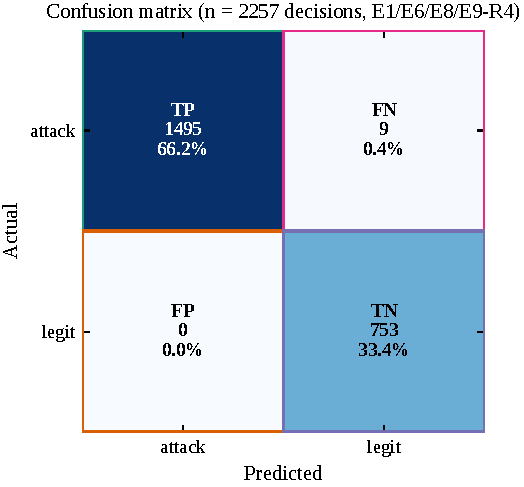
\includegraphics[width=0.85\columnwidth]{figures/fig_confusion_matrix.pdf}
  \caption{Pooled confusion matrix across the four scoring experiments
  (E1 attack detection, E6 oversize, E8 stochastic, E9 R4 evasion;
  $n = 2257$ decisions). Zero false positives and nine false negatives;
  the nine FNs come from the stochastic trials of E8 and match its
  recall of~\EEightstochasticRecallMean{}. E4 is an arbiter ablation
  (RAT disabled), not a detector-scoring run, so it is excluded from the
  pooled detector matrix.}
  \label{fig:cm}
\end{figure}

\begin{figure}[pos=htbp]
  \centering
  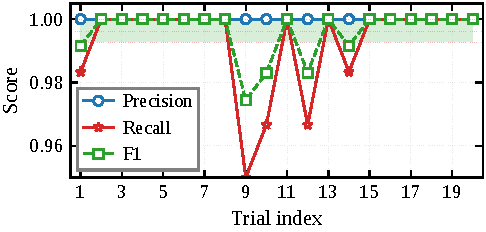
\includegraphics[width=\columnwidth]{figures/fig_per_experiment.pdf}
  \caption{Per-trial precision, recall, and F\textsubscript{1} across
  the \EEightstochasticNTrials{} stochastic E8 trials, with the
  F\textsubscript{1} bootstrap 95\% CI band shaded. The narrow
  dispersion shows that stochastic performance stays close to the CI
  interval reported for E8 in Table~\ref{tab:results}.}
  \label{fig:per_exp}
\end{figure}

\paragraph{Benign operational rollout (E12).}\label{sec:e12}
E12 answers the dual of the attack experiments: does the arbiter clear
rollouts that an operator is entitled to run? The workload drives six
legitimate patterns through Gate~A and Gate~B
(\S\ref{sec:rat-gates-6a}--\ref{sec:rat-gates-6b}). The backbone is a
five-wave staged rollout (ten BMSes per wave, 30~s between waves, 65~s
pause to clear the R5 window), and on top of that: an emergency hotfix
push that re-hits the same BMS inside R1's 14\,400~s window; two
migration sub-scenarios that switch the authorized source mid-rollout;
a delayed retry burst that compresses a staged wave into a few seconds;
a rollback preamble that primes each BMS's version high-water mark; and
a benign authorized rollback that downgrades the fleet by one version
under an explicit \texttt{rollback\_window} RAT entry. Every event is
labelled \textsc{legit}, so PASS is the correct verdict throughout.

\begin{figure*}[pos=htbp]
  \centering
  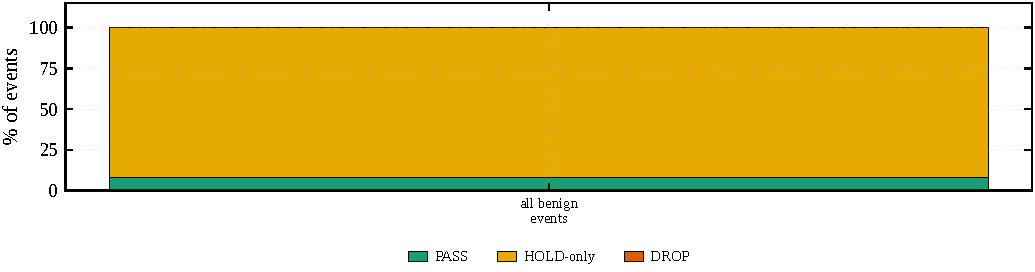
\includegraphics[width=0.55\textwidth]{figures/fig_benign_rollout.pdf}
  \caption{E12 aggregate outcome across
  \EOneTwobenignrolloutScenarioTotal{} legitimate events
  (\EOneTwobenignrolloutNTrials{} trials) on the deployed gated build.
  Classify-only silent PASS (no rule fired) covers
  \EOneTwobenignrolloutScenarioPass{} events; the remaining
  \EOneTwobenignrolloutScenarioHoldOnly{} events trip R1 (and R6 on
  authorized rollbacks) and are demoted to PASS by Gate~A
  (\EOneTwobenignrolloutScenarioGateA{}) or Gate~B
  (\EOneTwobenignrolloutScenarioGateB{}). No legitimate event fires R5:
  its fanout counter is gated on the unauthorized-source flag
  (\S\ref{sec:cascade-fix}), so authorized rollouts never reach it. Zero
  legitimate events are dropped.}
  \label{fig:benign_rollout}
\end{figure*}

Across \EOneTwobenignrolloutNTrials{} trials (Fig.~\ref{fig:benign_rollout}) the arbiter produced
\EOneTwobenignrolloutScenarioDrop{} DROPs on
\EOneTwobenignrolloutScenarioTotal{} legitimate events
(\EOneTwobenignrolloutScenarioFinalPassPct{}\% PASS):
\EOneTwobenignrolloutScenarioPass{} silent PASSes (no rule fired) and
\EOneTwobenignrolloutScenarioHoldOnly{} HOLD-only demotions, the latter
being packets that tripped a data-plane rule and were cleared by the
control-plane gate. On the deployed gated build the per-rule tally is
simple: \EOneTwobenignrolloutScenarioGateA{} events fire R1 (a re-push
inside R1's window) and are demoted to PASS by Gate~A, and
\EOneTwobenignrolloutScenarioGateB{} authorized rollbacks fire R1+R6 and
are demoted by Gate~B under an explicit \texttt{rollback\_window} RAT
entry. No legitimate event fires R5 (it is r2-gated,
\S\ref{sec:cascade-fix}), so the benign rollouts produce no
false positives. The three trials are a
reproducibility probe rather than a statistical sample (the scenario is
deterministic by construction), so the 0/450 FP count is reported with a
Clopper--Pearson one-sided 95\% upper bound of
\EOneTwobenignrolloutFPupperCP{}\% (at most that fraction of legitimate
events could be mislabelled at the 95\% confidence level) rather than as
an empirical point estimate. No rule-group produced a false positive.

\paragraph{Signed-manifest fail-safe (E12b).}\label{sec:e12b}
E12b validates the signed-manifest path end-to-end under controlled
tampering. Each of \EOneTwobsignedNTrials{} trials has two phases:
Phase~A runs a benign rollout under a valid ed25519-signed RAT; Phase~B
injects a single-byte flip on the detached signature file, forcing the
controller's hot-reload to reject the update and continue serving the
LKG manifest. Across Phase~A the arbiter processes
\EOneTwobsignedPhaseAEvents{} events with \EOneTwobsignedPhaseAFP{}
DROPs (FP-rate \EOneTwobsignedPhaseAFPrate{}); across Phase~B the LKG
manifest holds
\EOneTwobsignedPhaseBPass{}/\EOneTwobsignedPhaseBEvents{} events at
PASS, so the tampered reload never corrupts policy state. The stale-RAT
precision failure mode (expired \texttt{valid\_window}, no replacement
installed) is a distinct lifecycle condition discussed in the RAT
lifecycle matrix (\S\ref{sec:rat-lifecycle}).

\subsection{RQ2: Arbiter and R6 necessity}\label{sec:rq-ablation}

\noindent\textit{Finding: the RAT arbiter is necessary for admitting
authorized operations, not for attack precision. It clears the authorized
rollouts that trip the replay rule R1 (E12, zero benign-rollout false
positives) and the operator rollbacks that R6 would otherwise drop (E19,
Gate~B), and R6 is the sole detector of unauthorized rollback (removing it
makes rollback attacks invisible, E19). Disabling the arbiter leaves attack
precision unchanged (E4), because the data-plane terminal rules carry
attack detection.}

RQ2 establishes the arbiter's necessity on the operations it admits, the
benign rollouts of E12 (\S\ref{sec:rq-detection}) and the operator
rollbacks of E19 below, and isolates R6 as the sole rollback detector. The
attack-side sanity check (E4) comes last.

\paragraph{R5 gating and the deployed-build verdict.}\label{sec:cascade-fix}
On the deployed build the fleet-fanout counter (R5) is gated on
\texttt{r2\_fired}, and R2 is a terminal DROP that the policy engine
resolves before the R5 branch. R5 therefore never produces an independent
verdict over R2: it contributes fleet-fanout \emph{telemetry} rather than a
distinct line-rate action. The per-source \texttt{hold\_armed\_reg} gate
arms only on R5, so behind the terminal R2 drop it does not arm on any
reachable input and is inert (\S\ref{sec:known-correctness}). The
operational consequence is that an authorized rollout which trips the
per-BMS replay rule (R1) or the rollback rule (R6) reaches the arbiter and
is admitted, rather than being dropped at line rate before arbitration. The
defended space is therefore unauthorized-source campaigns and unauthorized
rollbacks, not arbitrary coordinated fanout from an already-authorized
source; that blind spot is stated in \S\ref{sec:discussion}. We keep the
gating because it removes benign-rollout false positives, at the cost of
R5's marginal independent detection, a trade we judge correct for an OT
deployment where a single false quarantine of a legitimate rollout is
operationally expensive.

This is the configuration under which E12, E19, and \Enineteenp{} are
measured: E12 (\EOneTwobenignrolloutNTrials{} trials,
\EOneTwobenignrolloutScenarioTotal{} legitimate events) reports zero
benign-rollout false positives, and \Enineteenp{}
(\EOneNineprollbackstochasticNTrials{} stochastic trials) reports precision
\EOneNineprollbackstochasticPrecisionMean{} (Wilson 95\% CI
$[\EOneNineprollbackstochasticPrecisionCIlo{},
\EOneNineprollbackstochasticPrecisionCIhi{}]$) and strict recall
\EOneNineprollbackstochasticRecallMean{} (Wilson 95\% CI
$[\EOneNineprollbackstochasticRecallCIlo{},
\EOneNineprollbackstochasticRecallCIhi{}]$). The strict recall counts
first-contact rollbacks, which R6 structurally cannot catch because a first
contact to a BMS has no stored version high-water mark, as misses
(\EOneNineprollbackstochasticFirstContact{} of
\EOneNineprollbackstochasticTotalMissed{} missed attacks); lenient recall
excluding them is \EOneNineprollbackstochasticRecallLenientMean{}. We
report the strict figure (rationale in \S\ref{sec:e19p}); R6's
first-contact blind spot is a scope limitation addressed in
\S\ref{sec:discussion}, with a baseline-warmup or cross-source version
prior as the natural mitigation.

\paragraph{Rollback ablation (E19).}\label{sec:e19}
A targeted ablation confirms that R6 is the sole rollback detector and
that disabling it cannot be compensated by R1 alone. With R6 enabled,
the arbiter produces \EOneNinerollbackRecallMean{} recall and
\EOneNinerollbackPrecisionMean{} precision over
\EOneNinerollbackLatencyN{} unauthorized rollback events across
\EOneNinerollbackNTrials{} trials (median end-to-end latency
\EOneNinerollbackLatencyMedianMs{}~ms). With R6 disabled, detection
collapses to \EnineteenAblationDetectionPct{}\%: across
\EnineteenAblationRollbackEvents{} rollback ground-truth events in
\EnineteenAblationNTrials{} ablation trials, the detector produced
\EnineteenAblationDrops{} DROPs. R1 alone cannot catch a v48$\to$v47
regression because R1 is a sliding-window inter-update test, not a
version-monotonicity test; only R6 enforces the high-water mark.

\paragraph{Stochastic rollback (\Enineteenp{}).}\label{sec:e19p}
\Enineteenp{} runs the unauthorized-rollback experiment with three axes
resampled per trial under independent RNG seeds: rollback
delta~$\sim$~\textsc{Uniform}(9, 16), benign-to-attack event
ratio~$\sim$~\textsc{Uniform}(0.3, 0.7), and inter-packet gap
$=$~20~ms~$+$~$\mathcal{N}(0, 15~\text{ms})$ clipped to $[10, 200]$~ms.
Across \EOneNineprollbackstochasticNTrials{} trials on the deployed gated
build the detector reports precision~$=$~%
\EOneNineprollbackstochasticPrecisionMean{}
[\EOneNineprollbackstochasticPrecisionCIlo{},
\EOneNineprollbackstochasticPrecisionCIhi{}] (Wilson 95\% CI; zero benign
false positives across \EOneNineprollbackstochasticEventLegit{}
legitimate events, Clopper--Pearson one-sided 95\% upper bound
\EOneNineprollbackstochasticFPupperCP{}\%) and strict
recall~$=$~\EOneNineprollbackstochasticRecallMean{}
[\EOneNineprollbackstochasticRecallCIlo{},
\EOneNineprollbackstochasticRecallCIhi{}], where strict recall counts a
first-contact no-decision as a miss. Of the
\EOneNineprollbackstochasticEventAttack{} rollback attacks the detector
drops \EOneNineprollbackstochasticEventTP{}; the
\EOneNineprollbackstochasticTotalMissed{} misses split into
\EOneNineprollbackstochasticEventFN{} reachable misses and
\EOneNineprollbackstochasticFirstContact{} first-contact rollbacks that
R6 structurally cannot catch, because a first contact to a BMS leaves no
stored version high-water mark to compare against. Excluding those
cold-start cases gives a lenient recall of
\EOneNineprollbackstochasticRecallLenientMean{}
[\EOneNineprollbackstochasticRecallLenientCIlo{},
\EOneNineprollbackstochasticRecallLenientCIhi{}]; we headline the strict
figure, in line with evaluation-integrity guidance for security
detectors~\cite{pendlebury2019tesseract,arp2022dosdonts}. Because a false
quarantine of a legitimate rollout is operationally more costly than a
missed cold-start rollback in this setting, we also summarise the
operating point with a precision-weighted
F\textsubscript{$\beta$}~($\beta = 0.5$, van
Rijsbergen~\cite{vanrijsbergen1979information}):
F\textsubscript{0.5}~=~\EOneNineprollbackstochasticFhalfStrict{} at strict
recall and \EOneNineprollbackstochasticFhalfLenient{} at lenient recall.
The strict recall reflects R6's first-contact blind spot rather than a
detection regression. Controller-side
(stage-2) detection latency:
\EOneNineprollbackstochasticLatencyMedianMs{}~ms median (p95
\EOneNineprollbackstochasticLatencyPninefiveMs{}~ms); adding the E14
stage-1 measurement ($\approx$29.5~ms) gives end-to-end
$\approx$40.2~ms. Per-trial outcomes and the first-contact recall
taxonomy are in Appendix~\ref{app:e19p-firstcontact}.

\paragraph{Arbiter ablation (E4), a sanity check.}\label{sec:e4}
For completeness we confirm the converse: the arbiter is not needed for
attack precision. Running the E1 workload against a controller launched
with \texttt{--disable-rat} (which forces every HOLD to DROP) leaves
precision at \EFourablationPrecisionMean{} and recall at 1.0, a change of
$\Delta$\,precision~=~\EfourAblationPrecisionDiffPP{}\,pp over
\EFourablationNTrials{} trials. Every drop is a terminal R1/R2 fire, and no
decision is a HOLD the RAT clears, because R5 is gated on
\texttt{r2\_fired} and never charges on an authorized rollout. The
arbiter's value is in admission (E12, E19), not attack precision.

\subsection{RQ3: Adversarial robustness}\label{sec:rq-adversarial}

\noindent\textit{Finding: adversaries who shape traffic around each
rule's threshold can escape the data plane:
\EOneSevenmimicryStrategyCaught{}/\EOneSevenmimicryStrategyTotal{}
(\EOneSevenmimicryStrategyCatchPct\%) of mimicry events are dropped, and
the residual blind zones are reported per rule below
(Fig.~\ref{fig:co-equal}).}

RQ3 asks how each rule degrades when an adversary is free to choose
attack parameters near the rule's detection boundary or to slow-play an
attack across a realistic deployment horizon.

\begin{figure}[pos=htbp]
  \centering
  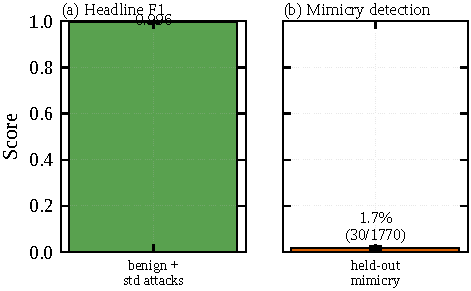
\includegraphics[width=0.92\columnwidth]{figures/F11_co_equal_headline.pdf}
  \caption{The two headline numbers, shown co-equal on a common
  $[0,1]$ scale: (a)~naive fleet-fanout detection
  F\textsubscript{1}~=~\EEightstochasticFOneMean{} (E8) versus
  (b)~adaptive-mimicry coverage \EOneSevenmimicryStrategyCatchPct\%
  (E21). The headline applies to the designed naive family; an adversary
  who reshapes cadence faces the right-hand number.}
  \label{fig:co-equal}
\end{figure}

\paragraph{Adversarial evasion sweeps (E9).}\label{sec:e9}
E9 probes the detection boundaries of R1, R4, and R5 by varying the
attack parameter across the threshold edge. \emph{R5 sweep:} fanout
sizes \{3, 4, 5, 6, 7, 10, 15, 20\} with disjoint BMS ranges and
65-second pauses; the transition from no-fire to fire occurs at
fanout~5, matching the compile-time threshold of~4
(count~$> 4 \Rightarrow$ fire). Above the threshold, P(R5 fires) grows
as $(N - 4) / N$ (Fig.~\ref{fig:r5}), confirming the rule's intrinsic
$\text{count} > 4$ boundary. This sweep characterizes R5's counter logic
directly; on the deployed build that counter is gated on
\texttt{r2\_fired}, so an \emph{authorized} fleet rollout never increments
it and never fires R5 (\S\ref{sec:cascade-fix}). The authorized-rollout
PASS rate is therefore 1.0 trivially: there is no R5 fire for the arbiter
to demote, not because the arbiter clears an R5 HOLD.
\emph{R4 sweep:} flow sizes \{1.5, 1.99, 2.0, 2.01, 4.0, 8.0\}~MiB; R4
fires only at and above 2.0625~MiB, the first size whose upper-16-bit
field reaches the range-match threshold (the data-plane compare is
\texttt{session\_bytes[31:16]}~$\geq 33$, i.e.\ $33 \times 64$~KiB). The
nominal oversize threshold is 2~MiB ($32 \times 64$~KiB), but the 64~KiB
quantization of the upper-16-bit key means a flow does not trip until it
crosses 2.0625~MiB; the 2.0 and 2.01~MiB sweep points fall inside this
$[2.0, 2.0625)$~MiB dead zone and do not fire. This is a documented
limitation of the range-match encoding.
\emph{R1 sweep:} inter-replay intervals \{10, 14399, 14400,
14401\}~seconds; R1 fires at intervals $\leq 14399$~s and does not fire
at $\geq 14400$~s, confirming the exact boundary. The 16-bit
wrap-around creates a theoretical false-positive window at 18.2-hour
multiples (\S\ref{sec:discussion}).

\begin{figure}[pos=htbp]
  \centering
  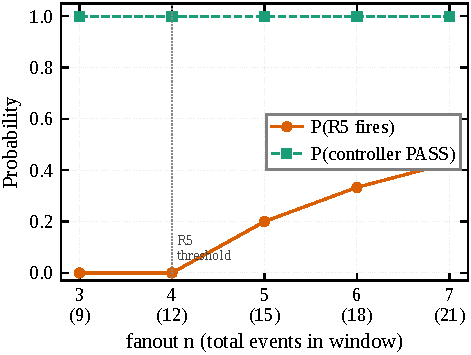
\includegraphics[width=0.85\columnwidth]{figures/fig_r5_boundary.pdf}
  \caption{R5 sensitivity as a function of fanout size: P(R5 fires) grows
  linearly above threshold 4, characterizing the rule's intrinsic counter.
  On the deployed build R5's counter is r2-gated, so an authorized fanout
  never fires R5 (\S\ref{sec:cascade-fix}); the authorized-rollout PASS
  rate is 1.0 trivially, with no R5 fire to demote.}
  \label{fig:r5}
\end{figure}

\paragraph{R1 behavior at high traffic rates.} Under E7's traffic
profile (one PUBLISH per 2~s mean across 50~BMSes), the mean per-BMS
revisit interval is approximately 100~s, far below R1's 14\,400~s
threshold. R1 therefore fires on the vast majority of legitimate
baseline packets. This is by design: R1 targets deployments where
individual BMSes receive firmware at most once per maintenance window
(hours to days), not continuous streaming. The threat model
(\S\ref{sec:background}) assumes infrequent OTA updates; E7 demonstrates
what happens when that assumption is violated, and its FP rate should be
interpreted as a sensitivity bound, not an operational FP measurement.

\paragraph{Per-strategy adaptive mimicry (E21).}\label{sec:e21}
E21 probes each rule's documented blind zone with five near-threshold
attack strategies, each labelled \textsc{attack} and emitted in its own
campaign over \EOneSevenmimicryNTrials{} repetitions
(\EOneSevenmimicryStrategyTotal{} attack events total). Each strategy is
emitted in isolation with a controller state reset between strategies so
that the drop, if any, is attributable to the strategy's own target
rule; a shared campaign instead lets one strategy's rule fire arm the
per-source hold register and cascade drops onto later same-source
strategies (\S\ref{sec:limitations}), which inflates the apparent catch
rate. The strategies are: (i) \emph{fanout-sub} keeps fanout at exactly
4 per 60~s window across six disjoint BMS groups so R5 does not fire;
(ii) \emph{fanout-three} fans a rollout to three BMS, one below the R5
threshold; (iii) \emph{R4 dead-zone} uses payload sizes inside the
range-match dead zone so R4 does not fire; (iv) \emph{combined} mixes
sub-threshold fanout with the R4 dead zone; (v) \emph{R1 late-replay}
re-hits the same BMS with a second replay in each pair.

\begin{table}[pos=htbp]
  \centering
  \caption{E21 rule-fire breakdown per mimicry strategy under
  per-strategy isolation, summed over \EOneSevenmimicryNTrials{}
  campaigns (\EOneSevenmimicryStrategyTotal{} attack events total).
  Each strategy is designed to evade a specific data-plane rule;
  ``caught'' counts events the controller dropped, ``missed'' counts
  everything else. Under isolation, only \emph{R1-late} produces any
  drop; every sub-threshold strategy evades entirely. Missed events
  escape the data plane and would need control-plane or endpoint
  recovery.}
  \label{tab:mimicry}
  \footnotesize
  \begin{tabular}{@{}l r r r r r r r@{}}
    \toprule
    Strategy & N & R1 & R2 & R4 & R5 & caught & missed \\
    \midrule
    fanout-sub    & 720 &  0 &  0 &  0 &  0 &  0 & 720 \\
    fanout-three  & 540 &  0 &  0 &  0 &  0 &  0 & 540 \\
    R4-deadzone   &  90 &  0 &  0 &  0 &  0 &  0 &  90 \\
    combined      & 360 &  0 &  0 &  0 &  0 &  0 & 360 \\
    R1-late       &  60 & 30 &  0 &  0 &  0 & 30 &  30 \\
    \midrule
    Total         &\EOneSevenmimicryStrategyTotal{}& 30 & 0 & 0 & 0
                  &\EOneSevenmimicryStrategyCaught{}
                  &\EOneSevenmimicryStrategyMissed{} \\
    \bottomrule
  \end{tabular}
\end{table}

The per-strategy fire counts are in Table~\ref{tab:mimicry} and the
per-strategy detection rates in Fig.~\ref{fig:mimicry}. R5 fires on zero
of the 720 fanout-sub and 540 fanout-three events,
confirming the sub-threshold-fanout blind zone on the hardware; R4 fires
on zero of the 90 dead-zone events, confirming the range-match blind
zone. Under per-strategy isolation the only strategy with any detection
is \emph{R1-late}, where R1 fires on the second replay of each pair
(\EOneSevenmimicryRoneLateCaught{}/\EOneSevenmimicryRoneLateTotal{},
\EOneSevenmimicryRoneLateRate{}); the \emph{combined} strategy, which a
shared continuous campaign had scored as dropped at a usable rate, is in
isolation fully evasive (0/360), confirming that the earlier apparent
catch was the per-source hold cascade rather than a target-rule fire.
Across all strategies the data plane drops only
\EOneSevenmimicryStrategyCaught{} of
\EOneSevenmimicryStrategyTotal{} attack events
(\EOneSevenmimicryStrategyCatchPct\%); the cross-strategy F1 is
\EOneSevenmimicryFOneMean{}
[\EOneSevenmimicryFOneCIlo{},~\EOneSevenmimicryFOneCIhi{}]. The residual
\EOneSevenmimicryStrategyMissed{} events pass the data plane without a
drop. These are the rule set's blind zones under adversarial input design;
endpoint signature verification and operator-side rollout monitoring remain
needed to close them.

\begin{figure}[pos=htbp]
  \centering
  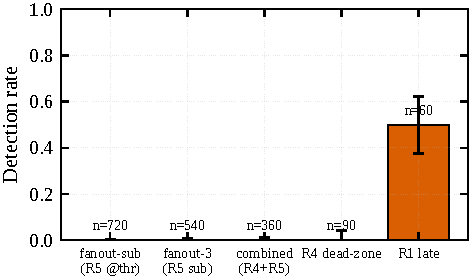
\includegraphics[width=0.92\columnwidth]{figures/F6_mimicry_per_strategy.pdf}
  \caption{E21 per-strategy adaptive-mimicry detection rate over
  \EOneSevenmimicryNTrials{} campaigns; error bars are Wilson 95\% CIs.
  Only \texttt{r1-late} produces any detection (R1 on the second replay,
  \EOneSevenmimicryRoneLateRate{}); every sub-threshold strategy evades
  entirely (0/N with Wilson upper bounds $<\!5\%$). Cross-strategy BCa
  F\textsubscript{1}~=~\EOneSevenmimicryFOneMean{}
  [\EOneSevenmimicryFOneCIlo{},~\EOneSevenmimicryFOneCIhi{}].}
  \label{fig:mimicry}
\end{figure}

\paragraph{TCP-segmentation evasion battery (E23).}\label{sec:e23-tcp}
The data plane parses the MQTT/OTA header per packet; it performs no TCP
reassembly. We measure the consequence directly with a $5\times5$
battery: five segmentation evasions against the five header-dependent
rules, 10 trials per cell (250 trials), each cell emitted after a
controller reset so the outcome is attributable to the cell's own rule.
Figure~\ref{fig:tcp-evasion} reports the observed per-cell drop rate. The
three \emph{header-split} evasions (\texttt{split-mqtt-fh},
\texttt{split-topic}, \texttt{split-ota-hdr}) cut the single
OTA-carrying PUBLISH across two segments so that no segment presents a
parseable header; all three evade \emph{every} rule, including the
source-keyed R2 (0.00 across the row), because R2's evaluation is gated
on the same per-packet OTA parse that the split defeats. The
\texttt{out-of-order} evasion (halves sent tail-first) likewise evades
every parse-dependent rule (R1/R4/R5/R6 $=0.00$) while R2 survives
($1.00$), since its first-sent segment still begins with the MQTT
control byte. Only \texttt{retransmit-dup}, which leaves an intact
PUBLISH on the wire, yields parse-dependent detection, and only
probabilistically (R1~$0.40$, R4~$0.60$, R6~$0.80$). No cell fires a
rule the threat model did not predict, so no evasion induces a spurious
drop. The R5 column is not a faithful fanout test (its single-PUBLISH
base attack cannot reach the $\geq 4$-BMS fanout threshold even
un-evaded), so its entries are shown for completeness, not read as
fanout-evasion results. The practical consequence: an adversary who
fragments the OTA PUBLISH at the TCP layer defeats the header-dependent
rules wholesale, so a stateful upstream reassembly point (or a
reassembling endpoint check) is required to close this class.

\begin{figure}[pos=htbp]
  \centering
  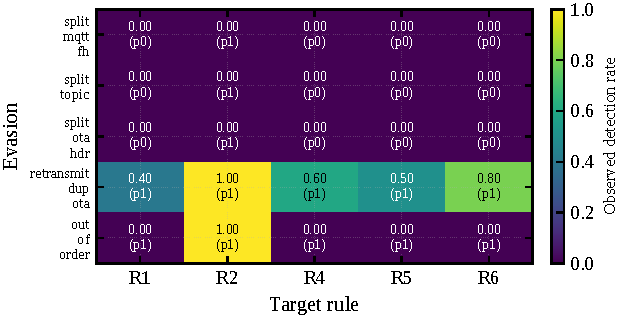
\includegraphics[width=0.92\columnwidth]{figures/F15_tcp_evasion.pdf}
  \caption{E23 TCP-segmentation evasion battery: observed per-cell drop
  rate over 10 trials/cell (250 trials), each cell reset-isolated; cell
  text is observed rate (predicted in parens). Header-split evasions
  defeat every rule including the source-keyed R2; only
  \texttt{retransmit-dup} (intact PUBLISH on the wire) yields
  parse-dependent detection, and only probabilistically. The R5 column
  does not exercise genuine fanout (single-PUBLISH base attack) and is
  shown for completeness.}
  \label{fig:tcp-evasion}
\end{figure}

\paragraph{Long-horizon slow-cadence trace (E7b).}\label{sec:e7b}
E7b runs the deployed gated build over a realistic deployment horizon:
\EsevenbNEvents{} events (\EsevenbNBenign{} benign updates plus
\EsevenbNAttack{} rollback attacks) over \EsevenbDurationHours{}~h of wall
clock, with per-BMS cadence resampled from \EsevenbCadenceKs{}~ks (median
inter-update interval $\approx$20{,}000~s). Two effects show up. First, the
slow cadence does not by itself silence the behavioral rules.
\EsevenbBenignObserved{} of the \EsevenbNBenign{} benign updates reach the
controller (the other \EsevenbBenignNoDecision{} pass natively at the data
plane with no decision); R1 fires on all
\EsevenbBenignRoneFires{} of them, where interleaved re-hits fall inside
its window, and the arbiter demotes each to PASS through Gate~A. R5 fires
on \EsevenbBenignRfiveFires{} benign updates, since it is r2-gated
(\S\ref{sec:cascade-fix}). No benign update is dropped
(\EsevenbBenignDrops{} false positives across \EsevenbNBenign{} updates;
precision \EsevenbOverallPrecision{}), consistent with the
0/\EOneTwobenignrolloutScenarioTotal{} of E12 (\S\ref{sec:e12}). Second, R6
catches all \EsevenbAttackRsixCatches{} of \EsevenbNAttack{} rollback
attacks (recall \EsevenbTPR{}, F1 \EsevenbOverallFOne{}). Unlike
\Enineteenp{}, this trace has no first-contact misses: over the long horizon
each BMS receives a benign update that establishes its version high-water
mark before any rollback targets it, so R6 always has a baseline to compare
against. E7b therefore complements \Enineteenp{}. Where \Enineteenp{}
isolates the cold-start gap with stochastic first-contact rollbacks
(\S\ref{sec:e19p}), E7b shows that once baselines are warm the deployed
build sustains P~=~R~=~F\textsubscript{1}~=~1.000 across an 8~h trace, with
the arbiter containing every benign rule fire.

\subsection{RQ4: CPU-based IDS baselines}\label{sec:rq-baseline}

\noindent\textit{Finding: off-the-shelf Suricata and Zeek fire on the
fanout shape of legitimate rollouts and cannot suppress it, so they
plateau at precision~0.67--0.70 on the same traffic where \otashield{}
reaches 1.00. \otashield{}'s edge is that R5 is gated in the data plane on
unauthorized sources, so authorized rollouts never fire it, while the RAT
arbiter demotes the R1 re-pushes that do fire. The gap is the policy-aware
pipeline, not baseline expressiveness.}

Conventional CPU-based IDS, Suricata and Zeek, run on the same
port-mirrored traffic a programmable switch can tee, so they are the
natural apples-to-apples baseline for an OTA detector that otherwise
requires a \tofino{} pipeline. RQ4 replays one E1 PCAP through five
baseline configurations that together span the expressive ceiling
reachable without a policy-aware arbiter.

\paragraph{CPU-based IDS baselines (E10).}\label{sec:e10}
We captured a PCAP of a single E1 trial (\EtenSuricataNDecisions{}~events:
60 attack + 30 legitimate) and replayed it through four baseline
configurations plus one apples-to-apples combination. R6 is omitted from
this mapping because the E1 PCAP contains no version-rollback events;
the R6 evaluation is reported separately in E19.
Table~\ref{tab:e10variants} collects the six variants; the text below
summarizes the arbitration gap they expose.

\begin{table}[pos=htbp]
  \centering
  \caption{E10 CPU-IDS baselines on the E1 PCAP replay
  (\EtenSuricataNDecisions{}~events: 60 attack + 30 legitimate).
  Variants (i)--(iv) are CPU-IDS configurations; variants~(v) and~(vi)
  post-process variants~(i) and~(iii)'s alerts respectively through the
  same RAT arbiter \otashield{} uses in-band (the apples-to-apples
  controls).}
  \label{tab:e10variants}
  \footnotesize
  \begin{tabular}{@{}l c c c c c@{}}
    \toprule
    Variant & Prec. & Recall & Acc. & TP & FP \\
    \midrule
    (i) Suricata min-effort        & N/A                               & \EtenSuricataRecall            & \EtenSuricataAccuracy          & 0  & 0 \\
    (ii) Suricata stateful         & \EtenSuricataStatefulPrecision    & \EtenSuricataStatefulRecall    & \EtenSuricataStatefulAccuracy  & \EtenSuricataStatefulTP & \EtenSuricataStatefulFP \\
    (iii) Suricata permissive      & \EtenSuricataPermPrecision        & \EtenSuricataPermRecall        & \EtenSuricataPermAccuracy      & \EtenSuricataPermTP     & \EtenSuricataPermFP \\
    (iv) Zeek domain-aware         & \EtenZeekPrecision                & \EtenZeekRecall                & \EtenZeekAccuracy              & \EtenZeekTP             & \EtenZeekFP \\
    (v) Suricata + RAT             & N/A                               & \EtenSuricataRatRecall         & \EtenSuricataRatAccuracy       & \EtenSuricataRatTP      & \EtenSuricataRatFP \\
    (vi) Suricata permissive + RAT & \EtenSuricataPermRatPrecision     & \EtenSuricataPermRatRecall     & \EtenSuricataPermRatAccuracy   & \EtenSuricataPermRatTP  & \EtenSuricataPermRatFP \\
    \bottomrule
  \end{tabular}
\end{table}

Variant (i) maps R1, R2, R4, R5 to the closest Suricata~7.0.3 primitive
(threshold, content byte match, dsize) and produces zero alerts; it is
retained as the expressive-floor anchor. Variant (ii) uses Suricata's
richer stateful primitives: \texttt{xbits(track ip\_dst, expire 14400)}
for per-destination replay memory, \texttt{flowint} accumulators for
byte totals, \texttt{threshold by\_src count 5, seconds 60} for R5
fanout, a negated allow-list for R2, and \texttt{flow:established} to
avoid matching synthetic mid-flow packets. Variant (iii) is the same
ruleset with \texttt{flow:established} relaxed to upper-bound what
Suricata rule primitives can express on a synthetic PCAP; it catches
every attack but flags every legitimate rollout that trips the same R5
fanout primitive. Variant (iv) replaces the rule DSL with a
script-based Zeek detector: a per-destination \texttt{last\_seen} table
(14\,400\,s expiry) for R1, a per-source fanout set (60\,s tumbling
window) for R5, an OTAS magic parser for payload inspection, and an R2
authorized-source check. Variant~(v) post-processes variant~(i)'s
Suricata alerts through the same RAT arbiter the \otashield{} controller
runs in-band, giving a rule-DSL detector access to RAT-based demotion.
Because variant (i) emits zero alerts on E1, the arbiter receives zero
inputs, and the combined system yields recall~=~0: giving a rule-DSL
detector access to RAT-based demotion does not rescue the expressive
floor when the rules themselves never fire. Variant~(vi) closes that
gap by arbitrating the alerts from variant~(iii) (which actually fire)
through the same RAT arbiter. Precision climbs to
\EtenSuricataPermRatPrecision{} (the RAT demotes every false-positive
legitimate-rollout alert), but recall drops to
\EtenSuricataPermRatRecall{}: half the attack events share the
authorized source IP and payload-size envelope of a legitimate rollout,
and the RAT arbiter, operating purely on Suricata's 5-tuple~+~timestamp
view, cannot distinguish a rapid-replay attack from a benign rollout on
the same flow key without per-flow R1/R4 bits. This is exactly the
signal \otashield{} keeps in the data plane: the arbiter upgrades
HOLD~$\to$~PASS or HOLD~$\to$~DROP using the rule set that fired on
\emph{this} flow, not a post-facto coincidence of 5-tuple and time
window. Giving a CPU-IDS baseline the RAT as a black-box post-filter
helps precision but silently drops half the attacks.

The pattern across variants (ii)--(iv) is consistent: once the baselines
receive the long-horizon state and cardinality primitives needed to
catch the attack events, they also flag every legitimate rollout that
happens to ride the same primitive. Stateful Suricata and domain-aware
Zeek both reach R~=~0.78--1.00 but plateau at P~=~0.67--0.70 because
neither can tell an authorized rollout from a campaign. \otashield{}
avoids these false positives in two ways the baselines cannot: R5 is gated
in the data plane on unauthorized sources, so an authorized fleet fanout
never fires it, and the RAT arbiter demotes the R1 re-pushes that do fire.
This is a policy-awareness gap, not an expressive gap: the detector
primitives are reachable on CPU; the data-plane authorization gating and
the rule-to-policy arbitration that suppress the legitimate-rollout fires
are not. R6 remains
inexpressible in Suricata's rule DSL in all variants; the Zeek variant
approximates it with the OTAS parser but still cannot distinguish
authorized rollbacks from unauthorized ones without RAT-equivalent
policy state.

\paragraph{Variant (vii): CPU port of the \otashield{} rule
arbiter.}\label{sec:e10-cpu-port}%
To isolate the in-network performance advantage from the rule
expressiveness advantage, we wrote a Python reference implementation of
the exact R1--R6 logic and RAT-aware arbitration the data-plane binary
executes. On the same \EtenSuricataNDecisions{}-event E1 PCAP, the CPU
port produces $P=R=F_1=1.00$ (TP=60, FP=0, TN=30, FN=0), matching the
data-plane binary exactly. Sustained throughput on a single CPU core is
$\sim 7\!\times\!10^{5}$~packets/s in unoptimized Python on three
captures of 90, 4841, and 7310 packets respectively. Compared against
the \tofino{} binary's line-rate forwarding budget on a 25~GbE port
(\(\sim 3.7\!\times\!10^{7}\)~pkt/s at 64~B), the CPU port is roughly
50$\times$ slower. The expressiveness gap from
variants~(i)--(vi) collapses to zero once the CPU detector implements
the same arbitration we run in the data plane; the remaining gap is
performance and resource cost, not detection quality. This separation
of concerns motivates \S\ref{sec:rq-cost} (latency, throughput,
capacity, portability), where the in-network deployment is justified on
cost rather than on detection ceiling.

\paragraph{Symmetric comparison on the full E8 population.}\label{sec:e10-symmetric}%
The E10 comparison above runs each baseline once on the single-trial E1
PCAP (90 events), whereas the headline OTA-Shield result (E8) uses 20
stochastic trials totalling \EEightstochasticEventTotal{} events. To
match sample size, we reconstructed a per-trial PCAP from each E8
stochastic trial (same packet format: scapy PA-only, MQTT/OTAS headers
from the recorded event parameters) and ran Suricata stateful-permissive
(the best-recall variant~(iii)) across all \EtenSymNTrials{} trials. The
pooled result on \EtenSymNEvents{} events (\EtenSymTP{} TP,
\EtenSymTN{} TN, \EtenSymFP{} FP, \EtenSymFN{} FN) is
P~=~\EtenSymPrecision{}, R~=~\EtenSymRecall{},
F\textsubscript{1}~=~\EtenSymFOne{}, identical to the single-trial E1
number, confirming that the asymmetry was in sample size, not in the
methodological conclusion. The stochastic ordering and ephemeral port
variation in the E8 trials do not alter Suricata's decision for any
event: variant~(iii)'s rules fire on every attack event and on every
legitimate rollout regardless of inter-arrival order, because neither
R1's \texttt{xbits} expiry nor R5's per-source threshold distinguishes
ordering within the 60-second window. Compared with OTA-Shield's E8
result (P~=~\EEightstochasticPrecisionMean{},
R~=~\EEightstochasticRecallMean{},
F\textsubscript{1}~=~\EEightstochasticFOneMean{}), the precision gap is
$\Delta P = \EEightstochasticPrecisionMean{} - \EtenSymPrecision{} =
0.333$ and the recall gap is 0. The \EtenSymFP{} false positives are 600
legitimate rollout events that Suricata's stateful rules flag on their
fanout shape and cannot demote, having no notion of an authorized
rollout. \otashield{} does not flag them at all, because R5 is r2-gated
(\S\ref{sec:cascade-fix}). On this workload the precision
advantage is therefore a \emph{data-plane} property, the r2-gating of R5,
not a control-plane demotion. The arbiter's complementary role shows up on
the per-BMS replay cohort: where a legitimate rollout instead trips R1 (a
re-push inside its window), Gate~A is what admits it, as E12 demonstrates
directly.

\begin{figure*}[pos=htbp]
  \centering
  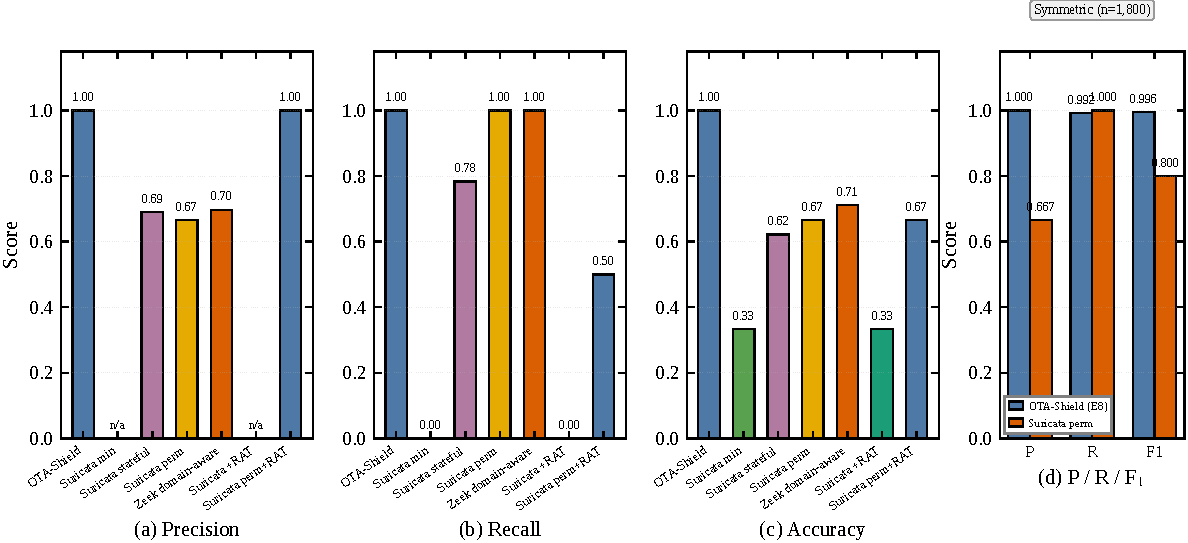
\includegraphics[width=0.95\textwidth]{figures/fig_suricata_vs_ours.pdf}
  \caption{CPU-based IDS baselines vs.\ \otashield{}.
  \textbf{Panels~(a)--(c): asymmetric comparison on the E1 PCAP replay}
  (\EtenSuricataNDecisions{} events: 60 attack + 30 legitimate), seven
  systems, three metrics. The minimum-effort Suricata mapping and its
  RAT-arbitrated combination (variant~v, apples-to-apples) both floor at
  recall~=~0; stateful Suricata and Zeek domain-aware recover recall to
  0.78--1.00 but plateau at precision~=~0.67--0.70 because they fire on
  the shape of legitimate rollouts and cannot suppress it. Variant~(vi) =
  permissive Suricata~+~RAT reaches precision~=~1.00 but its recall drops
  to \EtenSuricataPermRatRecall{} because RAT without per-flow R1/R4 bits
  cannot separate same-source rapid-replay attacks from legitimate
  rollouts. \otashield{} reaches P~=~R~=~1.00 on the same PCAP. The gap is
  policy-awareness, not the expressive power of any single primitive:
  \otashield{} gates R5 on unauthorized sources in the data plane and
  demotes R1 re-pushes at the arbiter.
  \textbf{Panel~(d): symmetric comparison on the full E8 population}
  (\EtenSymNEvents{} events across \EtenSymNTrials{} stochastic trials):
  Suricata stateful-permissive achieves P~=~\EtenSymPrecision{},
  R~=~\EtenSymRecall{}, F\textsubscript{1}~=~\EtenSymFOne{};
  \otashield{} achieves P~=~\EEightstochasticPrecisionMean{},
  R~=~\EEightstochasticRecallMean{},
  F\textsubscript{1}~=~\EEightstochasticFOneMean{}. Precision gap
  $\Delta P = 0.333$; recall gap $= 0$.}
  \label{fig:suricata}
\end{figure*}

\subsection{RQ5: Latency, throughput, capacity, and portability cost}\label{sec:rq-cost}

\noindent\textit{Finding: median latency is
\EEightstochasticLatencyMedianMs{}~ms (p95
\EEightstochasticLatencyPninefiveMs{}~ms), the override table holds
under sustained install pressure, and \EeighteenMfourMissed{} of
\EeighteenMfourVariants{} parser variants miss on a single-MQTT-profile
sweep. Costs land well inside the operational envelope.}

RQ5 reports the cost side of the ledger: end-to-end and per-stage
detection latency (E14 on the E8 dataset), controller-side digest
ingestion rate (E11), session-override table capacity (E13), and the
parser's sensitivity to MQTT-profile variations (E18).

\paragraph{Detection latency and per-stage breakdown (E14).}\label{sec:e14}
\begin{figure*}[pos=htbp]
  \centering
  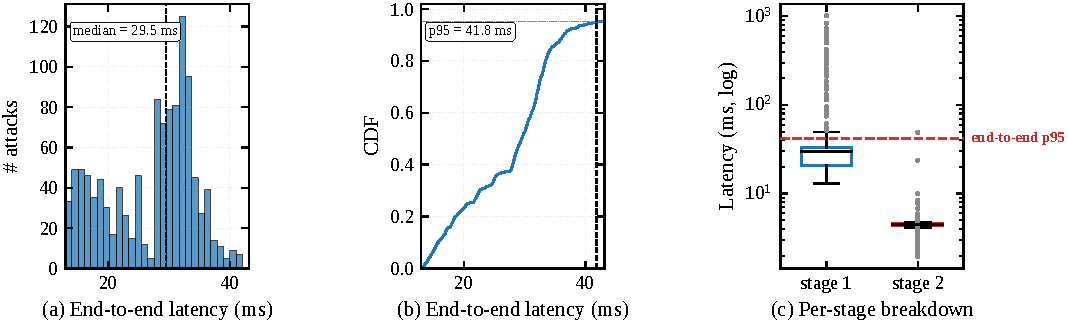
\includegraphics[width=0.88\textwidth]{figures/fig_detection_latency.pdf}
  \caption{End-to-end detection latency on \EEightstochasticLatencyN{}
  attack events from the stochastic experiment: (a)~histogram,
  (b)~empirical CDF, (c)~per-stage box plot on log scale. Stage~1 = send
  $\to$ digest arrival (generator + \tofino{} pipeline + gRPC transport);
  stage~2 = digest arrival $\to$ controller decision (Python
  arbitration); end-to-end = stage~1 + stage~2. Medians
  29.5/4.5/\EEightstochasticLatencyMedianMs{}~ms; p95 values
  41.8/4.8/\EEightstochasticLatencyPninefiveMs{}~ms. Latency is
  restricted to attack events because the benign workload interposes
  inter-trial state-reset barriers ($\sim$2.7~s) between trials; those
  barriers are driver-side synchronization, not per-event detection
  latency, so pooling them would overstate the on-path tail.}
  \label{fig:latency}
\end{figure*}
Using the timestamps already written to the E8 logs we decompose
end-to-end latency into two measurable stages on the
\EEightstochasticLatencyN{} attack events reported in
Fig.~\ref{fig:latency}. Stage~1 (send time $\to$ controller-side digest
arrival) captures the packet's flight from the generator plus the \tofino{}
pipeline plus the gRPC digest transport. Stage~2 (digest arrival $\to$
controller decision) captures the RAT arbitration path on the Python
side. Medians are stage~1~$=$~29.5~ms and stage~2~$=$~4.5~ms, and the
additive end-to-end median is therefore
\EEightstochasticLatencyMedianMs{}~ms = 29.5~ms + 4.5~ms (within the
0.1~ms rounding the macro carries). At p95 the two stages contribute
41.8~ms and 4.8~ms for an end-to-end p95 of
\EEightstochasticLatencyPninefiveMs{}~ms (= 41.8 + 4.8 within rounding).
The per-stage breakdown makes explicit that \emph{``in-switch''} does
not mean \emph{``in-switch latency''}: the dominant term is stage~1
(generator emission + \tofino{} pipeline + gRPC transport), and the ASIC
pipeline itself is a microsecond-scale component inside that
$\approx$29~ms envelope. Stage~2 contributes a small but non-negligible
4.5~ms tail to every decision because the controller's RAT-arbitration
path is Python and runs synchronously on digest receipt; stage~2 is the
largest software-side optimization target if a tighter SLA is required.
The latency distribution has a short head and a small tail. The tail is
driven by two infrequent controller-side events: a state-reset barrier
between trials, during which digest processing pauses briefly; and a
timer-based override-TTL sweep that contends with the main digest loop
for the gRPC channel when many session overrides expire at once. Neither
event is on the path of a data-plane fire-to-detection decision; both
affect when the controller's Python loop returns to the digest receive
call after the barrier. For an operational SLA measured in seconds (OTA
campaigns run over minutes to hours), this tail is tolerable; for a
tighter SLA, moving timer-driven override expiry out of the main thread
would flatten it.

\paragraph{Controller digest-channel sustainable rate (E11).}\label{sec:e11}
E11 measures the controller's classify/MQTT-parse digest ingestion path
(phases 1 and 2), not the phase-6 HOLD path: the generator sends MQTT
PUBLISHes to a destination outside the authorized BMS fleet with a
non-OTA topic prefix, so no rule fires and no override installs. The
pipeline still emits a phase-1 or phase-2 digest per parsed packet, and
it is this digest delivery the controller has to sustain. Sweeping
100/500/1000/2000~pps, the controller observed
\ElevenTotalObserved{}/\ElevenTotalSent{} digests for an aggregate loss
of \ElevenAggregateLossPct{}\% (worst per-rate \ElevenWorstLossPct{}\%
at 100~pps, statistical noise on the smallest window). The scapy
generator caps offered load near 2{,}200~pps, so this is a lower bound
on the controller's classify-digest rate, not an upper bound on switch
capability or on the HOLD-digest path. The HOLD-digest path is exercised
separately at the override-install rate measured in E13: every R5 fire
emits one phase-6 digest, the controller arbitrates, and installs at
most one override per source. ``No rule fires, no phase-6 digest, but a
classify/MQTT-parse digest still streams'' is the precise mapping
between E11's offered traffic and the measured digest count, and
resolves the apparent tension with the ``no rule fires $\Rightarrow$ no
digest'' phrasing used elsewhere, which referred specifically to
phase-6 HOLD digests. Line-rate testing of either path requires a DPDK
generator such as P4TG~\cite{lindner2023p4tg,ihle2025p4tgenhancements}
and is deferred to future work.

\paragraph{Override-table capacity (E13/T1.7).}\label{sec:e13}
The deployed \texttt{session\_action\_override} table keys on the full
5-tuple (\texttt{src\_addr}, \texttt{dst\_addr}, \texttt{dst\_port},
\texttt{protocol}, \texttt{src\_port}) and is sized at
\TOneSevenTableSize{} entries; we confirmed this key shape and size by
\texttt{bfrt\_grpc} inspection of the running pipeline on every trial of
T1.7. The 5-tuple key is a deliberate isolation property: an
\texttt{ALLOW} installed for one flow does not authorize unrelated traffic
from the same source, since an alias 5-tuple with different ports cannot
collision-match the entry. T1.7 measures the deployed table's capacity:
\TOneSevenNSources{} concurrent sources, one \texttt{ALLOW} each, install
cleanly across \TOneSevenNTrials{} trials (\TOneSevenTotalInserts{}
inserts in total) with \TOneSevenRejects{} \texttt{RESOURCE\_EXHAUSTED}
rejects (Clopper--Pearson 95\% upper bound \TOneSevenRejectUBPct{}\%), so
the \TOneSevenTableSize{}-entry table has headroom for a 200-source fleet
at one HOLD per source. The capacity that matters under this key is
\emph{5-tuple} cardinality, not source-IP cardinality: a single source
fanning out across many BMSes with churning ephemeral ports can generate
many distinct 5-tuples, which is why the table is paired with a 5~s
fail-closed TTL and why a source-IP aggregation variant is retained for
fanout-heavy deployments. The remainder of this paragraph reports that
variant.

\medskip\noindent\textit{Source-IP aggregation variant.}
The pilot 5-tuple-keyed override table at 1024 entries saturates within
seconds under sustained R5 fanout: a 1000~pps burst against 50 BMSes with
unique ephemeral source ports floods the table before the 5~s TTL can
evict stale entries. The aggregation variant instead keys on source IP
only, so every HOLD from one source collapses into a single table entry
regardless of how many BMSes the fanout covers. One override per source
covers that source's entire fanout until TTL expiry.

We run the install-pressure workload (sweep offered rate \{100, 250,
500, 1000\}~pps for 10~s, realized rate capped near
\EThirteenAggRealisedPpsMax{}~pps by the scapy raw-socket ceiling) from a
single authorized source. The E13 realized-rate ceiling
($\approx$500~pps) is lower than the E11 digest-channel ceiling
($\approx$2{,}200~pps) because the two workloads stress different
per-packet scapy costs: E11 sends a uniform PUBLISH stream to a single
unauthorized destination with no rule firing and no override install,
while E13 sweeps distinct source IPs and triggers a fresh R5 HOLD per
source that the generator must follow up with an install-ack bookkeeping
step. The per-frame encoding cost is therefore higher in E13, and the
same scapy raw-socket generator delivers a lower realised rate for the
same offered load. This is a property of the traffic shape and the
userspace generator, not a different hardware bound on the switch. Under
the aggregation variant, peak active override entries stay at
\EThirteenAggSingleSrcPeakActive{} across all four windows, despite
\EThirteenAggSingleSrcFiveTuples{} distinct 5-tuples in the largest
window. To measure the variant's cap on source-IP cardinality, we sweep
\{\EThirteenAggSrcSweepCounts{}\} distinct source IPs at 500~pps for 10~s
each (Fig.~\ref{fig:override_cap}). Peak active override entries track source-IP cardinality exactly
(\EThirteenAggSrcSweepPeakActives{}), and the switch records
\EThirteenAggSrcSweepRejects{} RESOURCE\_EXHAUSTED rejects across
\EThirteenAggSrcSweepTotalDecisions{} controller decisions. Table
occupancy is therefore bounded by source-IP cardinality, which typically
is 1--2 in a BESS fleet regardless of 5-tuple churn from ephemeral
ports. We retain this source-IP aggregation as a compile-time knob for
fanout-heavy deployments; the \emph{default in the deployed pipeline is
the 5-tuple-keyed table} characterised by T1.7 above, chosen for its
per-flow authorization isolation rather than for the lower occupancy of
the aggregation variant.

\begin{figure}[pos=htbp]
  \centering
  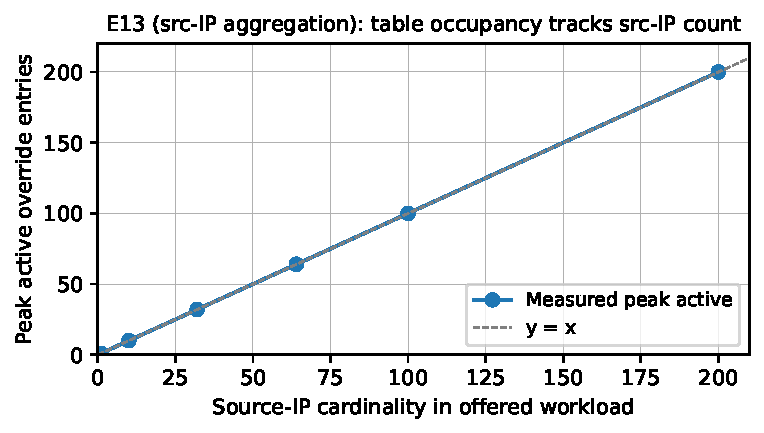
\includegraphics[width=0.88\columnwidth]{figures/fig_override_capacity.pdf}
  \caption{E13 (source-IP aggregation variant). Peak active
  override-table entries versus offered source-IP cardinality at
  500~pps per window, averaged over a 5~s TTL. Measurements fall exactly
  on $y=x$: one table entry per distinct source IP, independent of
  5-tuple fanout. Zero installs are rejected up to 200 source IPs in our
  deployment pipeline.}
  \label{fig:override_cap}
\end{figure}

\paragraph{Scope of the reference channel (E18).}\label{sec:e18}
E18 sweeps MQTT-level parameter variations (topic length, QoS level,
retain flag) to characterize how tightly the parser is bound to the
reference-channel assumptions. This is a scoping result rather than a
portability claim: it does not show that the construction ports to an
arbitrary MQTT profile, only that deviations from the reference framing
require per-channel re-engineering of the parser.
Table~\ref{tab:e18} reports the observed pipeline outcome per variant in
the core MQTT-parameter sweep.

\begin{table}[pos=htbp]
  \centering
  \caption{E18 reference-channel portability across the
  \EeighteenMfourVariants{}-variant MQTT-parameter sweep on the deployed
  parser. PARSED = the parser extracted a valid OTA header; PARSER-MISS =
  the packet was classified as non-OTA and forwarded unflagged. No variant
  is dropped; the determining factor is the 32-byte topic slot, not QoS or
  the retain flag.}
  \label{tab:e18}
  \footnotesize
  \begin{tabular}{@{}l l l@{}}
    \toprule
    Variant & Parameters & Outcome \\
    \midrule
    baseline      & topic=32~B, QoS=1, retain=0 & PARSED \\
    QoS=2         & topic=32~B, QoS=2, retain=0 & PARSED \\
    retain=1      & topic=32~B, QoS=1, retain=1 & PARSED \\
    QoS=0         & topic=32~B, QoS=0, retain=0 & PARSED \\
    short topic   & topic=16~B, QoS=1, retain=0 & PARSER-MISS \\
    long topic    & topic=64~B, QoS=1, retain=0 & PARSER-MISS \\
    QoS=0, short  & topic=16~B, QoS=0, retain=0 & PARSER-MISS \\
    QoS=0, long   & topic=64~B, QoS=0, retain=0 & PARSER-MISS \\
    \bottomrule
  \end{tabular}
\end{table}

The deployed parser parses every variant that keeps the 32-byte topic
slot (the reference channel and its QoS-2, retain, and QoS-0 variants) and
misses every variant that changes the topic length, which shifts the
OTA-header offset past the fixed slot. No variant is dropped, and QoS and
the retain flag do not affect parsing. This confirms that the OTA channel
used in the evaluation is a reference design rather than a universal model
of BESS OTA practice: an operational deployment on a different MQTT
profile would require a variable-length topic parser, which would add MAU
stages. This is consistent with the scope framing in
\S\ref{sec:intro}. Under the full \EeighteenMfourVariants{}-variant
sweep, the deployed binary parses
\EeighteenMfourParsed{}/\EeighteenMfourVariants{} variants end-to-end and
misses \EeighteenMfourMissed{} (all misses driven by topic-length
errors); agreement between the predicted and observed per-variant
outcome is \EeighteenMfourOk{}/\EeighteenMfourVariants{}. The single
disagreement is the QoS=0 variant at the reference 32-byte topic, which
parses observably even though the missing 2-byte packet identifier was
expected to misalign the OTA header: the deployed parser is more
tolerant of the QoS=0 offset shift than the byte layout suggests. The
practical implication is that the QoS=0 parser branch prepared for
recompile targets the variable-topic-length misses, which are
topic-length errors rather than QoS-offset errors. This does not affect
the headline portability claim
(\EeighteenMfourParsed{}/\EeighteenMfourVariants{} parse under the
current binary).

\paragraph{200-BMS fleet replay (E1$'$, E8$'$).}\label{sec:e1prime}
The reference numbers reported in
\S\ref{sec:rq-detection}--\ref{sec:rq-baseline} are bounded by a 50-BMS
testbed. To characterize the design at deployment-scale fleet size, we
replay two fleet-scale traces against the live controller. E1$'$ applies
a superposed-Poisson workload with \EOnePrimeNbms{} synthetic BMS
endpoints emitting \EOnePrimeIntendedEvents{} events at an aggregate
rate of 40~Hz. E8$'$ scales the stochastic E8 mix to the same fleet
size, producing \EEightPrimeIntendedEvents{} events. Per-BMS rate,
payload size, and version-bump probability are inherited from the
50-host long-baseline measurement; only fleet size and the synthetic
addresses 10.0.2.60--10.0.2.209 are extrapolated. Before the run, the
controller is restarted with the extended manifest so the override table
starts empty.

\begin{table}[pos=htbp]
  \centering
  \caption{50-BMS vs.\ 200-BMS precision and F\textsubscript{1}. Recall
  is preserved at 1.000 for both fleet sizes because detection coverage
  scales linearly with fleet size (the R1/R4/R6 rule chain is intact). The
  precision collapse at 200-BMS is attributed to the 64-entry
  controller/manifest BMS cap. The data-plane \texttt{bms\_ip\_to\_idx}
  table is itself compiled at 128 entries (Table~\ref{tab:mau-resource}),
  so legitimate packets addressed to BMS~65--200 are unmapped and take the
  fail-closed DROP path.}
  \label{tab:fleet-scaling}
  \small
  \begin{tabular}{@{}l c c c c@{}}
    \toprule
    Experiment & Fleet & Precision & Recall & F\textsubscript{1} \\
    \midrule
    E8 (50-BMS headline)  & 50  & \EEightstochasticPrecisionMean{} & \EEightstochasticRecallMean{} & \EEightstochasticFOneMean{} \\
    E1$'$ (200-BMS, det.)  & 200 & \EOnePrimePrecision{}           & \EOnePrimeRecall{}            & \EOnePrimeFOne{} \\
    E8$'$ (200-BMS, stoch.) & 200 & \EEightPrimePrecision{}         & \EEightPrimeRecall{}          & \EEightPrimeFOne{} \\
    \bottomrule
  \end{tabular}
\end{table}

The replay exposes two findings the 50-BMS workload cannot. First,
recall is preserved: across both scenarios no rollback attempt is missed
(\EOnePrimeFN{} and \EEightPrimeFN{} attack-side false negatives), so
detection coverage scales linearly with fleet size and the R1/R4/R6 rule
chain remains intact under sustained 40~Hz fanout. Second, the controller
caps the active BMS-index manifest at \PfourBmsIndexCap{} entries; the
data-plane \texttt{bms\_ip\_to\_idx} table itself is compiled at 128
entries (Table~\ref{tab:mau-resource}), so the bound here is operational,
not a hardware table-size limit. At 200~BMS the manifest cap leaves BMS
beyond the first \PfourBmsIndexCap{} unmapped: a legitimate packet
addressed to one of them misses the index table, is signalled
\texttt{action\_code}=2 by the data plane, and lands as a
\texttt{terminal\_fire} DROP at the arbiter. The aggregate result is
\EOnePrimePrecision{} precision and \EOnePrimeFOne{} F1 on E1$'$
(\EOnePrimeTP{} TP, \EOnePrimeTN{} TN, \EOnePrimeFP{} FP, \EOnePrimeFN{}
FN), and \EEightPrimePrecision{} precision and \EEightPrimeFOne{} F1 on
E8$'$. Digest loss at fleet scale is modest (\EOnePrimeDigestLossPct{}\%
on E1$'$, \EEightPrimeDigestLossPct{}\% on E8$'$), so the digest channel
itself is not the bottleneck.

The construction therefore holds at 200-BMS scale on the rule side but
not on the table-population side. The \PfourBmsIndexCap{}-entry cap is a
deployment-time scope rather than an algorithmic limitation: raising it to
the 128 the data-plane table already provides is a controller/manifest
change, and covering a fleet beyond 128 additionally requires a P4
recompile to widen the BMS-index, R1, and override tables, after which the
same controller and manifest cover the full fleet. We report
E1$'$ and E8$'$ alongside the 50-BMS numbers to make explicit which
result scales with fleet size (recall) and which depends on a recompile
(precision at fleet scale).

\FloatBarrier
%% ====================================================================
\section{Discussion and Limitations}\label{sec:discussion}

\subsection{Interpretation of results}

On the deployed gated build, E4 shows the terminal rules (R2, R4, R6)
carry the attack precision without the arbiter: disabling the RAT leaves
precision at 1.0, because R5 is gated on \texttt{r2\_fired} and never
fires on an authorized rollout. The arbiter's value is on rollback
admission (E19), not an R5 precision delta. The boundary sweeps (E9) map hardware-imposed
limits (R4's 64~KiB dead zone between 2.0--2.0625~MiB and R1's
18.2-hour wrap-around) into the threat model rather than hiding them. No
single rule is evasion-proof; the multi-rule architecture is
defense-in-depth within a reference channel. The remainder of this
section states the limitations we measured, and for each names a
realistic next step.

\subsection{Limitations}\label{sec:limitations}

The three deployment paths this scope implies were set out early in
Fig.~\ref{fig:scope} (\S\ref{sec:background}): a supported cleartext segment
after TLS/VPN termination, and two paths the evaluated build does not cover,
a brokered path (E20) and an encrypted or TCP-segmented path (E23). The
paragraphs below detail each.

\paragraph{TLS / VPN scope.} \otashield{} requires placement after
TLS/VPN termination or access to plaintext OTA metadata. The R1, R4, R5,
and R6 rules all read fields that the parser extracts from the cleartext
MQTT PUBLISH and the 20-byte OTA header; on a flow still inside a TLS or
VPN tunnel at the switch, the parser cannot recover any of those fields
and none of the rules can fire. The deployment requirement is therefore
that an upstream broker, IIoT gateway, or VPN concentrator terminate the
encrypted leg, and that \otashield{} sit on the cleartext segment
between the terminator and the BMS fleet. Next step: a cross-protocol
side-effect rule (R7) correlating post-flash bursts in NTP, DNS, and
DHCP, which would cover encrypted OTA channels whose payload cannot be
parsed.

\paragraph{Comparative-evaluation scope.} Our baseline comparison spans
two tiers run on our own traffic, off-the-shelf signature IDS (Suricata,
Zeek) and a CPU port of \otashield{}'s own rule and arbiter logic (E10),
plus a cited-numbers table positioning \otashield{} against prior
in-network and ICS detectors. We did not run a prior
ICS-specific IDS on our own PCAPs. The closest neighbour, a P4-MQTT
topic-enforcement detector~\cite{binh2026p4mqtt}, targets broker ACL
violations rather than OTA fleet coordination and runs on a software
(BMv2) target, so a like-for-like port onto the E1/E8 captures would
convert that prose positioning into a measured point. We leave that port
to future work.

\paragraph{Brokered-MQTT source-IP collapse (E20).}\label{sec:e20-broker}
Where the OTA path traverses an MQTT broker rather than reaching the
fleet directly, a topology some grid profiles mandate, every PUBLISH on
the BMS-facing wire carries the broker's source IP. We emulate this on
the testbed (80 trials $\times$ 30 publishes across one benign and three
attack scenarios, with post-relay packets carrying the broker source IP)
and the controller fires R2 (unauthorized
source) on all 600 of every scenario's events, benign and malicious
alike, dropping the benign broker-relayed rollout in full (600/600 false
positives). The source-IP-keyed rules cannot separate authorized from
rogue publishers once the broker collapses their addresses, so an
IP-only authorization table yields no precision in this topology
(negative control: precision collapses, F1 undefined under all-drop).
The mitigation is to key authorization on a publisher identity carried
end-to-end through the broker rather than on the source IP; the
data-plane header reserves a 64-bit hash-hint field for exactly this
purpose, but the controller-side publisher-id keying is not implemented
in the evaluated build. Brokered deployment is therefore a documented
gap: we report no
publisher-id F1, because with no publisher-id logic in the controller
any such number would reflect the IP-keyed all-drop behavior rather than
a working publisher-id RAT.

\paragraph{RAT trust surface.} Detection accuracy rests on a correct RAT
manifest. An attacker with write access before controller start, or a
privileged insider authoring entries, can widen a rollback window and
suppress R6 for that scope. Because Gate~B matches on
$(\mathit{src}, \mathit{dst}, \mathit{size}, \mathit{version})$ rather
than firmware content, a compromised authorized source can also inject an
image whose declared version falls inside a legitimate window, and a
sub-threshold fanout ($\leq 4$, which E21 shows fires R5 on
$0/1260$ events) carrying such a version passes both gates without ever
raising a HOLD. The mitigations are operational: short-lived per-rollout
entries, a signed manifest (the controller verifies an ed25519 signature
at load and hot-reload and retains the last-known-good cache on failure,
E12b Phase~B), bounded \texttt{rollback\_window} spans, and a
WARNING-level audit record on every Gate~B demotion. Signature
verification does not catch replay of an older valid manifest; binding
manifests into a monotonic chain is left to operator integration.

\paragraph{Per-source HOLD gate.}\label{sec:known-correctness} The
\texttt{hold\_armed\_reg} gate is indexed by the low 8~bits of a CRC16 of
the source IP (256 buckets). On the deployed build it arms only on R5, and
because R5's counter is gated on \texttt{r2\_fired} behind the terminal R2
drop, the gate does not arm on any reachable input and is inert; this is
why E12 and \Enineteenp{} report zero benign false positives. (An earlier
build armed the gate on any rule fire, which is the configuration recorded
in Appendix~\ref{app:build-provenance}.) The 256-bucket index remains a
latent limitation
for any future build that re-arms the gate on unauthorized fanout: at 10
to 50 concurrent sources, birthday collisions would make it unreliable as
a per-source discriminator, and widening the index to a 32-bit CRC32 over
the 5-tuple is the mitigation. Rollback detection (R6) further assumes a
prior reference version for the targeted BMS: an attack to a device with
no baseline yields a no-decision, so lenient recall is
\EOneNineprollbackstochasticRecallLenientMean{} over devices with an
established baseline and strict recall is
\EOneNineprollbackstochasticRecallMean{} counting first-contact
no-decisions as misses (\S\ref{sec:e19p},
Appendix~\ref{app:e19p-firstcontact}).

\paragraph{Bloom sizing for fleet fanout.}\label{sec:bloom-scaling} The R5
fanout detector indexes each destination into three 1024-entry Bloom
filters. Because it gates on \texttt{r2\_fired==1} (\S\ref{sec:impl}),
the load that matters is unauthorized fanout per 60-s window, not fleet
size, and the deployed sizing is collision-free for the fleet sizes
evaluated here. Sustained unauthorized fanout above that band would need
wider registers; a 4096-entry resize fits in SRAM without an added MAU
stage.

\noindent The remaining limitations, including the session-hash
collision bound (E5$'$), the cadence-gated status of R1 (E7), and the
override-table capacity evidence (E13), are summarised in
Table~\ref{tab:limits}.

\begin{table*}[pos=htbp]
  \centering
  \small
  \caption{Limitations of \otashield{} outside the RAT trust surface.
  Each row names a limitation, its blind zone or failure mode, and an
  available mitigation path.}
  \label{tab:limits}
  \begin{tabular}{@{}p{3.0cm}p{5.2cm}p{5.2cm}@{}}
    \toprule
    \textbf{Limitation} & \textbf{Blind zone / failure mode} & \textbf{Mitigation} \\
    \midrule
    Simulation conventions
      & Parser assumes 32-byte null-padded topics and QoS\,=\,1 with
        packet identifier; \EeighteenMfourMissed{} of
        \EeighteenMfourVariants{} swept variants miss the OTA header
        (E18).
      & Recirculation or a variable-length extraction pipeline;
        deployment-specific parser re-engineering per channel. \\
    \addlinespace
    Switch line-rate throughput
      & Measured ceiling is ${\approx}\,$2{,}200~pps on a scapy
        generator; \tofino{} line-rate is not exercised. Headline
        F\textsubscript{1} is bound to the generator, not to the ASIC.
      & DPDK-class traffic generator (P4TG) on dedicated ports, deferred
        to future hardware work. \\
    \addlinespace
    Testbed fidelity
      & 50 BMS endpoints share a single kernel, NIC, and clock;
        device-side jitter, clock skew, and per-device TCP behavior are
        not reproduced.
      & Evaluation on physical-device fleets; timing distributions not
        measured here. \\
    \addlinespace
    Session hash collisions
      & \MFiveHashBits-bit CRC32 index has birthday-bound collisions
        $\approx N(N{-}1)/2^{17}$; R4 can false-positive or
        false-negative under concurrent flows. E5$'$ confirms the
        analytical bound at $N{=}10\,000$ with
        \MFiveCollisionsTenThousand{} observed collisions
        (\MFiveRateTenThousandPct\%, vs.\ predicted
        \MFiveTheoRateObsTenKPct\%).
      & Wider index (20-bit, 1\,M entries) or set-associative table, at
        the cost of register memory. \\
    \addlinespace
    R1 cadence gating
      & R1 applies only when per-BMS cadence is slower than
        $\tau_{\mathrm{R1}} = 14\,400$~s; under faster cadences R1 fires
        on legitimate traffic (E7) and must be disabled.
      & R2, R4, R5, R6 carry detection under faster cadences;
        control-plane replay detection for streaming cadences. \\
    \addlinespace
    Threshold robustness
      & R5, R1, R4 thresholds are compile-time constants; no runtime
        adaptive thresholds.
      & By design: compile-time constants keep thresholds auditable and
        immutable; per-deployment recompile using E7 percentiles and E9
        sensitivity. \\
    \addlinespace
    Parser short-packet DoS
      & PUBLISHes with payload ${<}20$~bytes to OTA topics trigger a
        parser error and drop: fail-closed for attacks, but also drops
        legitimate short status messages.
      & Topic-prefix ACL upstream of the parser to scope fail-closed
        behavior. \\
    \addlinespace
    Override table capacity
      & \texttt{session\_action\_override} keys on the full 5-tuple
        (compile size 256); occupancy bounded by 5-tuple cardinality under
        ephemeral-port churn (T1.7: 4000 inserts across 200 sources, 0
        RESOURCE\_EXHAUSTED).
      & Compile-time size is the knob; a source-IP aggregation variant
        (occupancy bounded by source-IP cardinality, E13) is preserved for
        fanout-heavy deployments. \\
    \bottomrule
  \end{tabular}
\end{table*}

\subsection{Positioning relative to prior systems}

No prior system addresses the same combination of BESS OTA semantics,
in-pipeline data-plane enforcement, and policy-aware control-plane
arbitration, so numeric comparison carries caveats.
Table~\ref{tab:comparison} places \otashield{} alongside the closest
prior work by detection domain, platform, and headline metric. Each row
reports a number from the cited paper on that paper's own dataset; they
are not numbers from a common benchmark, and no single row is directly
comparable to ours.

\begin{table*}[pos=htbp]
  \centering
  \caption{Position of \otashield{} relative to related in-network
  detectors and CPU-based IDS. Each row reports a metric from the cited
  paper on \emph{that paper's own dataset}; the dataset column makes
  explicit that these are not measured on a shared benchmark, and the
  numbers are not comparable across rows. The \otashield{} row and the
  E10 CPU-IDS rows are the only rows measured on the same traffic as
  this paper.}
  \label{tab:comparison}
  \footnotesize
  \begin{tabular}{@{}l l l l@{}}
    \toprule
    System & Platform & Domain & Result on cited dataset (not comparable across rows) \\
    \midrule
    Raj \& Jin~\cite{samsonraj2025dddas}  & Tofino    & Dynamic-data ML IDS        & CICIDS: high accuracy \\
    Chen et al.~\cite{chen2024p4nids}     & Tofino    & P4 NIDS (distilled trees)  & authors' trace: low-SRAM pipeline \\
    AlSabeh et al.~\cite{alsabeh2022p4ddpi} & P4 sw.\ & DDoS entropy DPI           & authors' DDoS trace: in-paper metric \\
    Jaqen~\cite{liu2021jaqen}             & Tofino    & Volumetric DDoS            & authors' testbed: 380\,Gb/s mitigation \\
    MQTT pipeline~\cite{binh2026p4mqtt}   & BMv2 (soft) & MQTT enforcement         & authors' emulator: 99.8\% \\
    \midrule
    \multicolumn{4}{@{}l}{\textit{Measured on the E10 PCAP in this paper:}} \\
    Suricata~7 (stateful)~\cite{waleed2022whichids} & CPU & Signature IDS + xbits/flowint & E10 PCAP: P=0.69, R=0.78 \\
    Zeek (domain-aware)                   & CPU         & Script-based IDS          & E10 PCAP: P=0.70, R=1.00 \\
    \otashield{} (this work)              & \tofino{}    & BESS OTA fleet attacks    & E8 PCAP: F\textsubscript{1}\,\EEightstochasticFOneMean{}
      [\EEightstochasticFOneCIlo{}, \EEightstochasticFOneCIhi{}] \\
    \bottomrule
  \end{tabular}
\end{table*}

On the same PCAP we benchmarked four CPU-IDS configurations
(\S\ref{sec:e10}): a minimum-effort Suricata mapping (recall
\EtenSuricataRecall{}), a stateful Suricata mapping using
\texttt{xbits}/\texttt{flowint}/\texttt{threshold}
(P~=~\EtenSuricataStatefulPrecision{}, R~=~\EtenSuricataStatefulRecall{}),
the same mapping with \texttt{flow:established} relaxed as an expressive
upper bound (P~=~\EtenSuricataPermPrecision{},
R~=~\EtenSuricataPermRecall{}), and a Zeek domain-aware script-based
detector (P~=~\EtenZeekPrecision{}, R~=~\EtenZeekRecall{}). Variants
(ii)--(iv) all cluster at P~$\approx$~0.67--0.70 once they reach useful
recall. The bottleneck on a CPU IDS is not data-plane line rate or
detector expressiveness; it is that none of the CPU baselines can tell an
authorized rollout from a coordinated campaign. \otashield{} gets this
from two policy-aware mechanisms the baselines lack: R5's fanout counter
is gated in the data plane on the unauthorized-source flag, so authorized
rollouts never trip it, and the RAT arbiter demotes the legitimate
re-pushes that do fire R1. Its precision advantage at matched recall is
therefore a property of the policy-aware pipeline as a whole, chiefly the
data-plane r2-gating of R5 on this fanout workload, rather than of the
control-plane arbiter alone.

\subsection{Operational implications}

For BESS operators, \otashield{} provides a detection layer that
operates at the network aggregation point (between the OTA server and the
BMS fleet), where coordinated campaigns are visible but endpoint
protections are blind. The RAT enables scheduled rollouts to proceed
without false alarms, while the 5-second fail-closed override window
limits the exposure of any single detection miss. The compile-time
threshold constants require a P4 recompile to change (minutes, not
hours), which is consistent with planned maintenance cycles but not with
real-time threshold adaptation.

\subsection{Composing \otashield{} with endpoint and operator-side defenses}\label{sec:compose}

\otashield{} is one layer in a defense-in-depth stack, not a standalone
detector. Table~\ref{tab:layers} sketches what each layer catches and
misses.

\begin{table*}[pos=htbp]
  \centering
  \caption{Defence-in-depth coverage. Each layer catches a different
  fraction of the attack space; \otashield{} is one of the three, not a
  replacement for the others.}
  \label{tab:layers}
  \footnotesize
  \begin{tabular}{@{}l p{0.70\columnwidth}@{}}
    \toprule
    Layer & What it catches \\
    \midrule
    Endpoint signing (SUIT/Uptane) & Unsigned or mis-signed firmware at
      the BMS, regardless of how it arrives. Blind to
      \emph{signed-but-malicious} firmware (stolen signing key) and blind
      to in-transit fanout. \\
    \otashield{} data plane    & Naive coordinated campaigns (A1--A4 at
      their designed thresholds, plus A5 rollback via R6 and Gate~B) at
      the network aggregation point. Blind to shaped adversaries that
      stay inside rule blind zones (E21); requires placement after
      TLS/VPN termination (\S\ref{sec:discussion}). \\
    Operator rollout dashboard & Slow-drift campaigns visible over hours
      to days through fleet-version skew. Too slow to stop a
      minutes-scale attack in flight. \\
    \bottomrule
  \end{tabular}
\end{table*}

\subsection{Resource and deployment cost}\label{sec:cost}

Unlike CPU-based IDS, the data-plane layer pays its cost in MAU stages,
SRAM, and amortized switch hardware rather than in cores and watts.
Table~\ref{tab:cost} collects the measured resource footprint.

\begin{table*}[pos=htbp]
  \centering
  \caption{Resource footprint of \otashield{} on \tofino{}, with rough
  comparison to a CPU-based alternative on the same traffic.
  Dollar-per-BMS-year assumes a five-year amortization of a USD~20\,k
  switch over a 50-unit fleet.}
  \label{tab:cost}
  \footnotesize
  \begin{tabular}{@{}l l l@{}}
    \toprule
    Cost dimension & \otashield{} (\tofino{}) & Suricata (Xeon Gold) \\
    \midrule
    MAU stages used              & 12 of 12 (Table~\ref{tab:mau-resource}) & n/a \\
    SRAM for rule state          & 3\,KB (R5 Bloom) + 0.5\,KB (R1) & host RAM \\
    Session table (fleet-wide)   & 512\,KB (two 64\,K $\times$ 32\,bit) & host RAM \\
    Power per Gb/s (amortized)   & $\sim$70\,mW/Gb/s         & $\sim$5\,W/Gb/s \\
    Throughput headroom          & measured 2{,}200\,pps (generator-bound); ASIC 25\,Gb/s link, unmeasured & 40--60\,Gb/s~\cite{hu2019analysinghighspeed} \\
    Hardware cost (list)         & \$20\,k (32$\times$100\,GbE) & \$8--12\,k server \\
    \$/BMS-year (50-unit fleet)  & $\approx$\$80             & $\approx$\$40 \\
    \bottomrule
  \end{tabular}
\end{table*}

\begin{table*}[pos=htbp]
  \centering
  \caption{Per-component data-plane resource placement, extracted from the
  deployed build's compiler output (the \texttt{context.json}/BFA of the
  binary loaded by \texttt{bf\_switchd}). The pipeline occupies all 12
  ingress MAU stages. ``Largest match table'' gives the dominant logical
  table per component and its entry count; ``Stateful registers'' lists
  the SALU-backed memory. Exact chip-relative SRAM/TCAM percentages
  require the compiler's MAU resource log, which was not retained for the
  deployed binary; we therefore report the authoritative allocation
  counts.}
  \label{tab:mau-resource}
  \footnotesize
  \begin{tabular}{@{}l l l l@{}}
    \toprule
    Component & Stage(s) & Largest match table (entries) & Stateful registers (entries) \\
    \midrule
    Parsing + topic match    & 0      & \texttt{topic\_prefix} (8)              & --- \\
    Session manager          & 0--1   & \texttt{session\_id} (64\,K)            & \texttt{session\_bytes} (64\,K), \texttt{first\_ts} (64\,K), \texttt{coarse\_time} (1) \\
    R2 unauthorized source   & 1      & \texttt{r2\_authorized\_sources} (16)   & --- \\
    R5 fleet fanout          & 1--6   & \texttt{fleet\_monitor} (64\,K)         & \texttt{bf\_r0/r1/r2} ($3{\times}$1024), \texttt{r5\_count} (1) \\
    BMS index map            & 5      & \texttt{bms\_ip\_to\_idx} (128)         & --- \\
    R4 oversize              & 5--6   & \texttt{r4\_threshold} (range)          & shares \texttt{session\_bytes} \\
    R1 replay                & 6--7   & \texttt{secondary\_rules} (256)         & \texttt{r1\_last\_seen} (256) \\
    R6 rollback              & 6      & \texttt{rule\_r6\_rollback} (256)       & \texttt{r6\_bms\_max\_version} (256) \\
    Policy engine            & 7--8   & \texttt{set\_src\_idx} (256)            & --- \\
    Override + hold cascade  & 9--10  & \texttt{session\_action\_override} (256, 5-tuple) & \texttt{hold\_armed} (256) \\
    Deparser digests         & 11     & $6{\times}$ learn-quantum digests       & --- \\
    \midrule
    \multicolumn{4}{@{}l}{\textbf{Whole pipeline:} 12 of 12 ingress stages;
    76 PHV containers (23$\times$8\,b, 25$\times$16\,b, 28$\times$32\,b);
    14 SALU units; 10 TCAM blocks; 10 map RAMs.} \\
    \bottomrule
  \end{tabular}
\end{table*}

Table~\ref{tab:mau-resource} gives the per-component placement extracted
from the deployed build's compiler output. \otashield{} uses all 12
ingress MAU stages; the long pole is the chain of dependent rule state
(session bytes $\rightarrow$ R4/R5 thresholds $\rightarrow$ R1/R6 history
$\rightarrow$ policy $\rightarrow$ override), each link of which must
follow its producer's stage. The three range-match threshold checks (R1,
R4, R5) account for the TCAM use, and the stateful registers account for
the SALU use, notably the three 1024-entry R5 Bloom filters and the two
64\,K-entry session arrays. The full stage occupancy is the binding
constraint on adding rules: a seventh behavioral rule with its own
stage-dependent state would not fit without folding existing logic, which
is one reason new detection logic is added in the controller rather than
the data plane. (We also note that \texttt{bms\_ip\_to\_idx} is sized at
128 entries in the compiled table; the 64-BMS figure quoted elsewhere is a
controller/manifest-imposed cap, not the data-plane table size.)

Two caveats on the cost table. The switch cost is amortized over a single
50-unit fleet; in a larger substation with multiple fleets sharing the
switch, the per-BMS figure falls proportionally. The power comparison is
approximate: \tofino{} ASIC power is roughly constant (the pipeline cost
is marginal once the ASIC is on), while CPU IDS power scales with offered
load.

At the 50-unit fleet measured here, Suricata is roughly 2$\times$ cheaper
in \$/BMS-year at list prices; we report Table~\ref{tab:cost} as a direct
measurement at our evaluated scale rather than as a claim that
\otashield{} is cheaper per BMS in absolute terms. The in-network
deployment contributes performance headroom and co-location with the
forwarding path, not cost or unique detection capability at this fleet
size. Two regimes where the tradeoff may favor in-network placement are:
(a)~multi-fleet substations where the switch is amortized across hundreds
of BMS (e.g., a 200\,+ BMS substation, lowering the per-BMS cost to
${\approx}$\$20); and (b)~high-OTA-traffic loads where a CPU-bound IDS
would need per-packet reassembly at rates the ASIC handles with zero
incremental cost. Serving such a fleet means raising the 64-entry BMS
manifest cap (a controller change up to the 128 the table already holds)
and, beyond 128 BMS, a per-deployment P4 recompile to widen the index;
without that headroom precision collapses as measured in E1$'$
(\S\ref{sec:e1prime}). Quantifying the cost-parity
crossover point is deferred to future work with a DPDK-class traffic
generator.

\subsection{RAT manifest lifecycle}\label{sec:rat-lifecycle}

The RAT is not a hard-coded file. We sketch an operational pipeline: the
operator's firmware deployment system (for example, Ansible, GitHub
Actions, or a vendor portal API) emits a \texttt{rat.json} fragment per
rollout that is merged into the active manifest and loaded into the
controller on inotify hot-reload (or a 5-second polling fallback when
inotify is unavailable). Two distinct RAT failure modes are quantified.
First, integrity: under E12b's signed-manifest tamper test, a single-byte
flip on the detached signature is rejected by the controller and
last-known-good policy holds across
\EOneTwobsignedPhaseBPass{}/\EOneTwobsignedPhaseBEvents{} post-tamper
events with \EOneTwobsignedPhaseAFP{} false positives across
\EOneTwobsignedPhaseAEvents{} valid-signature events. The reload path is
therefore fail-safe. With kernel inotify enabled, across
\EOneTwobsignedNTrials{} trials the controller logged a
\texttt{RAT reload REJECTED} event in
\EOneTwobsignedRejectTrials{}/\EOneTwobsignedNTrials{} trials and
re-loaded the last-known-good manifest in \texttt{signed=True} mode in
\EOneTwobsignedSignedOkTrials{}/\EOneTwobsignedNTrials{} trials; the
controller never silently fell through to unsigned mode. The fail-safe
behavior itself is independent of the trigger-observation rate. Second,
freshness: a stale RAT (for example, a manifest 24~hours behind the
actual rollout schedule) degrades precision because genuine rollouts
fall outside the active time window, and the arbiter then converts their
R1 fires to DROP overrides. On a benign-only workload this is a pure-loss
failure mode: every R1 fire under a stale RAT is a false positive, so an
operator running on a stale manifest is worse off than one running with
the RAT disabled on the same benign workload. The lifecycle plumbing (signed
manifests, inotify hot-reload with polling fallback, stale-window
alerts) is therefore essential.

\paragraph{Lifecycle matrix (E22).}\label{sec:e22}
On the deployed gated build we re-ran the active-authorized lifecycle state
(signed RAT hot-reload, per-event reset, ten trials): all 80
authorized-rollout events PASS with zero false positives, reproducing E12.
The remaining four states of the original matrix (pre-rollout, post-expiry,
active-unauthorized off-target, and max-concurrent) probe enforcement the
deployed data plane does not perform: an authorized source
with a valid version, size, and target that deviates only in schedule or
concurrency carries no unauthorized-source or oversize signal, trips no
terminal rule, and is admitted rather than quarantined. This is the
documented R5-gating scope (the defended space is unauthorized-source
campaigns and unauthorized rollbacks, not off-parameter operation from an
already-authorized source, \S\ref{sec:cascade-fix}), and schedule freshness
is enforced at the manifest layer through E12b's signed-reload and
stale-window path (\S\ref{sec:e12b}), not by a data-plane rule. Two harness
constraints make a full deployed-build matrix uninformative: per-event
reset isolates single
packets, so the R5 fleet-fanout counter cannot fire by construction, and
although the controller enforces \texttt{max\_concurrent\_targets}
(\S\ref{sec:policy}), the per-event reset keeps the concurrent-session
count from accumulating, so the cap cannot be exercised in this harness.
We therefore report only the in-scope
active-authorized confirmation and do not treat the off-parameter states as
detection events; a containment-oriented matrix would require the
5-tuple-indexed hold register of \S\ref{sec:known-correctness} behind a P4
recompile, left to future work.

Rollback decisions ride the same lifecycle. Gate~B
(\S\ref{sec:rat-gates-6b}) expresses an authorized downgrade campaign as
an optional \texttt{rollback\_window} field on the per-rollout manifest
fragment, and inherits the manifest's signing and refresh pipeline. The
defaults favor the operator: a manifest without \texttt{rollback\_window}
entries keeps R6 terminal, and a stale or absent manifest degrades to
R6-as-terminal rather than silent suppression. Gate~B sits behind the
same signed-manifest boundary that Gate~A already relies on.

\FloatBarrier
%% ====================================================================
\section{Conclusion}\label{sec:conclusion}

We described \otashield{}, a hardware-measured reference architecture
for in-network detection of coordinated OTA firmware distribution
attacks against battery energy storage systems, implemented on an Intel
\tofino{} programmable switch. The design places an OTA parser and
fleet-cardinality counter on the transit path where endpoint signature
checks are blind, and a policy-aware control-plane arbiter (Gate~A,
Gate~B) that consults a Rollout-Authorization Table on a cleartext
segment after TLS or VPN termination.

On a 50-unit emulated BMS testbed the data-plane rules hold attack
precision at 1.0 without control-plane help (E4 ablation on the gated
build); the RAT arbiter's measured role is admitting operator-authorized
rollbacks that the version-monotonicity rule (R6) would otherwise drop
(E19).
The held-out mimicry study reports each rule's measured blind zone
(adaptive mimicry drops coverage to \EOneSevenmimicryStrategyCatchPct\% of attack events), and the
capacity sweep reports when the session-override table saturates under
sustained install pressure. The design also detects signed rollback
attempts through a per-BMS version-monotonicity rule (R6), with
authorized downgrade exceptions handled explicitly through Gate~B.

The contribution is the arbitration architecture: a data-plane rule set
gated so that authorized rollouts never reach the fanout counter, and a
RAT arbiter that admits the operator rollbacks the version rule would
otherwise drop. Two scopes bound the result. The
F\textsubscript{1}~=~\EEightstochasticFOneMean{} headline covers the
designed fleet-fanout family; an adversary who reshapes cadence faces the
\EOneSevenmimicryStrategyCatchPct\% mimicry coverage instead. Switch
line-rate is not measured here, and the end-to-end F\textsubscript{1} is
bound by a scapy generator ceiling of ${\approx}\,$2{,}200~pps. The
reference-channel profile, the cadence-gated R1, and the bounded Suricata
comparison are detailed in \S\ref{sec:discussion}.
Future work includes variable-length topic parsing, a set-associative
session table for larger fleets, held-out OTA-channel variants
(binary-diff firmware, broker-relayed MQTT, non-MQTT transports), and
operational integration with complementary telemetry monitoring. A
cross-protocol side-effect rule (R7) that correlates post-flash bursts
in NTP, DNS, and DHCP within a short window is a further extension that
would cover encrypted OTA channels whose payload we cannot parse.

%% CRediT statement -- withheld for double-blind review

%% Data availability (required)
\section*{Data availability}
Code and data will be released at an anonymized repository upon
acceptance; URL withheld for double-blind review.

%% Declaration of competing interests (required)
\section*{Declaration of competing interests}
The authors declare that they have no known competing financial
interests or personal relationships that could have appeared to
influence the work reported in this paper.

%% AI disclosure (required by Elsevier 2024 policy)
\section*{Declaration of generative AI and AI-assisted technologies in the writing process}
The author used AI-assisted coding tools to draft code and AI for basic
grammar correction. The author reviewed and edited all output and takes
full responsibility for the publication.

\FloatBarrier
\appendix
\section{E8 per-trial results}\label{app:e8-per-trial}

Table~\ref{tab:e8-per-trial} reports the raw per-trial outcomes for the
20 E8 stochastic trials summarized in \S\ref{sec:e8}. Across 20 trials
the detector produces $F_1 = 0.9962 \pm 0.0075$ (mean $\pm$ stdev; range
$[0.9744, 1.0000]$), with dispersion concentrated in three trials that
miss one to three of 60 attack events. Precision is exactly $1.0$ on
every trial. These numbers underlie the aggregated
\texttt{\EEightstochasticFOneMean{}} [\texttt{\EEightstochasticFOneCIlo{}},
\texttt{\EEightstochasticFOneCIhi{}}] result reported in the body;
readers who want to assess dispersion directly rather than rely on the
bootstrap CI can do so from this table.

\begin{table}[pos=htbp]
  \centering
  \caption{E8 per-trial confusion-matrix counts and derived metrics.
  TP/FN/FP/TN are raw event counts; precision, recall, and F1 are
  derived per-trial.}
  \label{tab:e8-per-trial}
  \footnotesize
  \begin{tabular}{@{}r r r r r r r r@{}}
    \toprule
    Trial & TP & FN & FP & TN & Precision & Recall & F1 \\
    \midrule
     1 & 59 & 1 & 0 & 30 & 1.0000 & 0.9833 & 0.9916 \\
     2 & 60 & 0 & 0 & 30 & 1.0000 & 1.0000 & 1.0000 \\
     3 & 60 & 0 & 0 & 30 & 1.0000 & 1.0000 & 1.0000 \\
     4 & 60 & 0 & 0 & 30 & 1.0000 & 1.0000 & 1.0000 \\
     5 & 60 & 0 & 0 & 30 & 1.0000 & 1.0000 & 1.0000 \\
     6 & 60 & 0 & 0 & 30 & 1.0000 & 1.0000 & 1.0000 \\
     7 & 60 & 0 & 0 & 30 & 1.0000 & 1.0000 & 1.0000 \\
     8 & 60 & 0 & 0 & 30 & 1.0000 & 1.0000 & 1.0000 \\
     9 & 57 & 3 & 0 & 30 & 1.0000 & 0.9500 & 0.9744 \\
    10 & 58 & 2 & 0 & 30 & 1.0000 & 0.9667 & 0.9831 \\
    11 & 60 & 0 & 0 & 30 & 1.0000 & 1.0000 & 1.0000 \\
    12 & 58 & 2 & 0 & 30 & 1.0000 & 0.9667 & 0.9831 \\
    13 & 60 & 0 & 0 & 30 & 1.0000 & 1.0000 & 1.0000 \\
    14 & 59 & 1 & 0 & 30 & 1.0000 & 0.9833 & 0.9916 \\
    15 & 60 & 0 & 0 & 30 & 1.0000 & 1.0000 & 1.0000 \\
    16 & 60 & 0 & 0 & 30 & 1.0000 & 1.0000 & 1.0000 \\
    17 & 60 & 0 & 0 & 30 & 1.0000 & 1.0000 & 1.0000 \\
    18 & 60 & 0 & 0 & 30 & 1.0000 & 1.0000 & 1.0000 \\
    19 & 60 & 0 & 0 & 30 & 1.0000 & 1.0000 & 1.0000 \\
    20 & 60 & 0 & 0 & 30 & 1.0000 & 1.0000 & 1.0000 \\
    \midrule
    mean & 59.55 & 0.45 & 0.0 & 30.0 & 1.0000 & 0.9925 & 0.9962 \\
    stdev &  0.89 & 0.89 & 0.0 & 0.00 & 0.0000 & 0.0148 & 0.0075 \\
    \bottomrule
  \end{tabular}
\end{table}

\section{\Enineteenp{} first-contact recall taxonomy}\label{app:e19p-firstcontact}

Rollback detection (R6) requires a prior authenticated reference version
for the targeted BMS: an attack packet to a device with no established
baseline produces a no-decision (ND) rather than a HOLD, because R6 has
no high-water mark to compare against. When a trial's Phase-1 baseline
covers fewer devices than the attack set targets, the uncovered devices
have no stored version, so attack packets to them generate a parse-level
digest rather than a HOLD digest and the controller makes no decision.
This is a fundamental property of a version-monotonicity detector, not a
tuning artifact. We report two recall framings on the deployed gated
build (\EOneNineprollbackstochasticEventAttack{} rollback attacks across
\EOneNineprollbackstochasticNTrials{} trials; the detector drops
\EOneNineprollbackstochasticEventTP{} of them):

\begin{description}
  \item[Framing~(i), ND-excluded (lenient).] Recall over attack events on
    devices with an established Phase-1 baseline:
    $\EOneNineprollbackstochasticEventTP{}/406 =
    \EOneNineprollbackstochasticRecallLenientMean{}$ (Wilson 95\% CI
    $[\EOneNineprollbackstochasticRecallLenientCIlo{},
    \EOneNineprollbackstochasticRecallLenientCIhi{}]$). This matches the
    detector's stated operating condition, a BMS whose baseline R6 has
    already recorded. The \EOneNineprollbackstochasticEventFN{} reachable
    misses are rollbacks that reached the controller but were not dropped.
  \item[Framing~(ii), strict (headline).] Counting the
    \EOneNineprollbackstochasticFirstContact{} first-contact ND events as
    false negatives:
    $\EOneNineprollbackstochasticEventTP{}/\EOneNineprollbackstochasticEventAttack{}
    = \EOneNineprollbackstochasticRecallMean{}$ (Wilson 95\% CI
    $[\EOneNineprollbackstochasticRecallCIlo{},
    \EOneNineprollbackstochasticRecallCIhi{}]$). This is the figure we
    headline, treating any undetected attack packet as a miss regardless
    of first-contact status, per evaluation-integrity guidance for
    security detectors~\cite{pendlebury2019tesseract,arp2022dosdonts}.
\end{description}

\noindent The first-contact ND rate is
$\EOneNineprollbackstochasticFirstContact{}/\EOneNineprollbackstochasticEventAttack{}$.
Precision is \EOneNineprollbackstochasticPrecisionMean{} with zero benign
false positives across \EOneNineprollbackstochasticEventLegit{}
legitimate events (\S\ref{sec:e19p}). The un-gated build's apparent
near-perfect recall was an artifact of the \texttt{hold\_armed\_reg}
cascade incidentally dropping first-contact rollbacks; on the deployed
gated build that cascade is inert (\S\ref{sec:cascade-fix}), so the
cold-start misses surface as the gap between strict and lenient
recall.

\section{Build provenance and the R5-gating revision}\label{app:build-provenance}

The results in this paper were collected on two successive binaries, and
this appendix records which experiment ran on which so that each number can
be tied to a fixed configuration. The deployed build gates the fleet-fanout
counter (R5) on the unauthorized-source flag (\texttt{r2\_fired}) and arms
the per-source \texttt{hold\_armed\_reg} gate only on R5; because R5 sits
behind the terminal R2 drop, that gate is inert on reachable input
(\S\ref{sec:cascade-fix}, \S\ref{sec:known-correctness}). An earlier
un-gated build armed the per-source gate on \emph{any} rule fire. On that
build a compressed benign rollout that tripped the per-BMS replay rule (R1)
would arm the gate and drop the source's subsequent packets at line rate
before the arbiter could clear them, producing benign-rollout false
positives. Restricting the gate's arming to R5 removes this behavior, and
E12, E19, and \Enineteenp{} were re-measured on the deployed build, where
they report zero benign-rollout false positives (\S\ref{sec:e12},
\S\ref{sec:e19p}).

One consequence of the revision is the rollback recall the deployed build
reports. The un-gated build recorded a near-perfect rollback recall, but
that figure was inflated: the per-source gate incidentally dropped
first-contact rollbacks that R6 itself cannot catch, because a first
contact to a BMS has no stored version high-water mark. On the deployed
build those cold-start cases surface as the gap between strict
recall (\EOneNineprollbackstochasticRecallMean{}, counting first-contact
events as misses) and lenient recall
(\EOneNineprollbackstochasticRecallLenientMean{}); we report the strict
figure (\S\ref{sec:e19p}, Appendix~\ref{app:e19p-firstcontact}).

The five-state lifecycle matrix (E22, \S\ref{sec:e22}) was originally
completed only on the un-gated binary, where the per-source gate pre-empts
the arbiter (152 of 160 benign rollout events dropped, a 95\%
false-positive rate). We re-ran the in-scope active-authorized state on the
deployed gated build (0 false positives across 80 events, confirming the
fix); the remaining states probe off-parameter authorized operation that
the gated build does not quarantine (\S\ref{sec:e22}), and a
containment matrix that also exercises a per-source hold role would require
the 5-tuple-indexed hold register of \S\ref{sec:known-correctness} behind a
P4 recompile. The integrity and freshness lifecycle failure modes are
covered by E12b (\S\ref{sec:e12b}). Table~\ref{tab:provenance} summarizes
the per-experiment configuration.

\begin{table}[pos=htbp]
  \centering
  \caption{Per-experiment build provenance. ``Deployed gated'' is the final
  binary (R5 r2-gated, per-source hold gate inert, 5-tuple-keyed override
  table); ``un-gated'' is the earlier binary used before the R5-gating
  revision. The last column marks whether the result is part of the
  deployed-build story or is auxiliary/motivating only.}
  \label{tab:provenance}
  \footnotesize
  \begin{tabular}{@{}l l l c@{}}
    \toprule
    Experiment(s) & Binary & R5 gating & Deployed story \\
    \midrule
    E1, E2, E6, E8, E14      & deployed gated & r2-gated & yes \\
    E4 (arbiter ablation)    & deployed gated & r2-gated & yes \\
    E12, E12b                & deployed gated & r2-gated & yes \\
    E19, \Enineteenp{}       & deployed gated & r2-gated & yes \\
    E9, E21, E23, E20        & deployed gated & r2-gated & yes \\
    E10 (incl.\ symmetric)   & deployed gated & r2-gated & yes \\
    E11, E13, E18            & deployed gated & r2-gated & yes \\
    E7b (long-horizon)       & deployed gated & r2-gated & yes \\
    \midrule
    E1$'$, E8$'$ (200-BMS)   & earlier binary & n/a      & scope only (cap-limited) \\
    E22 active-authorized    & deployed gated & r2-gated & yes (confirms fix) \\
    E22 full matrix          & un-gated       & ungated  & motivating only \\
    \bottomrule
  \end{tabular}
\end{table}

\noindent The override table is 5-tuple-keyed on the deployed build
throughout (\S\ref{sec:e13}); E13 additionally characterizes the optional
source-IP aggregation variant. E7b was re-run on the deployed gated build
(\S\ref{sec:e7b}): over the 8~h trace it records 0 benign false positives
and catches all 100 rollback attacks, so it now reports on the deployed
binary rather than an un-gated auxiliary run.

{\footnotesize
\setlength{\bibsep}{1pt plus 0.2ex}
\bibliographystyle{unsrtnat}
\bibliography{references}
}

\end{document}
